\documentclass[
  11pt,             % 10pt | 11pt | 12pt
  french,           % french | english
  %greyCover,        %
  fancyChapter,     %
  fancyPart,        %
  %squeezeCommittee %
]{these-LUNAM_mod}

%\usepackage{etex}            % solve compatibility issues
\usepackage[utf8]{inputenc}   %
\usepackage[T1]{fontenc}      %
\usepackage{textcomp}         % °, <<, >>, etc.
\usepackage{times}            %
\usepackage{natbib}           %
\usepackage{xifthen}          %
\usepackage{relsize}          % \mathlarger
\usepackage{multirow}         %
\usepackage{booktabs}         % \addlinespace, \toprul, \bottomrule, etc.
\usepackage{subfigure}        %
\usepackage{tikz}             %
\usepackage{pgfplots}         %
\usepackage{makeidx}          %
\usepackage{amsthm}           % theorem definition and styling
\usepackage{epigraph}         % chapter heading quote
\usepackage[inline]{enumitem} %
\usepackage{ragged2e}         % \justifying
\usepackage{rotating}         % \sideways in table

\usetikzlibrary{positioning, shapes, arrows, patterns}

\setlength\epigraphwidth{10cm}
\setlength\epigraphrule{0cm}

\RequirePackage[bookmarks,
                colorlinks,
                urlcolor=black,
                citecolor=black,
                linkcolor=black,
                hyperfigures,
                pagebackref,
                pdfcreator=LaTeX,
                breaklinks=true,
                pdfpagelayout=SinglePage,
                bookmarksopen=true,
                bookmarksopenlevel=2]{hyperref}

\geometry{inner=2.5cm, outer=2.5cm, top=2.5cm, bottom=2cm}
\geometry{inner=3.5cm, outer=3.5cm, top=4cm, bottom=3.5cm} % CUSTOM
%\geometry{inner=1.5cm, outer=1.5cm, top=2cm, bottom=2cm}

\setlist[enumerate]{itemsep=0mm}  % minimum spacing between items (it is not
\setlist[itemize]{itemsep=0mm}    % same as \setlist[...]{noitemsep}
\renewcommand{\labelitemi}{--}
\renewcommand{\labelitemii}{-}
\renewcommand{\labelitemiii}{-}
\renewcommand{\labelitemiv}{-}

%-------------------------------------------------------------------------------

\newcommand\chaptercite[2]{\epigraph{\justifying{\Large``}\textit{#1}{\Large''}}{--- #2}}
\newcommand\smallchaptercite[2]{\epigraph{\hfill{}{\Large``}\textit{#1}{\Large''}}{--- #2}}

\newcommand\ditto{$_{^\textnormal{\normalsize\textquotedbl}}$}

\renewcommand\cite[2][]{\ifthenelse{\equal{#1}{}}{\citep{#2}}{\citep[#1]{#2}}}
\newcommand\newcite[2][]{\ifthenelse{\equal{#1}{}}{\citet{#2}}{\citet[#1]{#2}}}

\newcommand\TODO[1]{\textcolor[rgb]{1, 0, 0}{[TODO #1]}}
\newcommand\REMARK[1]{\textcolor[rgb]{0, 1, 0}{[#1]}}

\theoremstyle{remark}
\newtheorem{example}{Exemple}

\makeindex

%%%%%%%%%%%%%%%%%%%%%%%%%%%%%%%%%%%%%%%%%%%%%%%%%%%%%%%%%%%%%%%%%%%%%%%%%%%%%%%%

\titre{Indexation automatique par termes-clés\\de documents en domaines de spécialités}
%\soustitre{}

\title{Automatic Domain-Specific Keyphrase Annotation}
%\subtitle{}

\author{M.}{Adrien}{Bougouin}

\discipline{Informatique}                             %
\sectionCNU{27}                                       % Informatique
\specialty{Traitement automatique du langage naturel} %


\institution{UN} % - UN, UA, UM, ECN, MN (formerly EMN), Oniris, Agro
%\coinstitution[10pt]{<description>}{<acronyme>}{2.4cm}
%\cosupervisingforeigninstitution[10pt]{<description>}{<acronyme>}{3.2cm}

\doctoralschool{Sciences et technologies de l'information, et mathématiques}
%\europeanlabel
\laboratory{Laboratoire d'informatique de Nantes-Atlantique (LINA)}
%\thesisnumber{}
\date{28 septembre 2015}


%% DEFENSE COMMITTEE %%%%%%%%%%%%%%%%%%%%%%%%%%%%%%%%%%%%%%%%%%%%%%%%%%%%%%%%%%%

\reviewer{}{}{}{}{}
\reviewer{}{}{}{}{}
%\reviewer{<civilité>}{<prénom>}{<nom>}{<titre>}{<établissement>}
% absent during defense
%\reviewer*{<civilité>}{<prénom>}{<nom>}{<titre>}{<établissement>}

%\president{<civilité>}{<prénom>}{<nom>}{<titre>}{<établissement>}
%\examiner{<civilité>}{<prénom>}{<nom>}{<titre>}{<établissement>}
% absent during defense
%\examiner*{<civilité>}{<prénom>}{<nom>}{<titre>}{<établissement>}

%\guest{<civilité>}{<prénom>}{<nom>}{<titre>}{<établissement>}

%-------------------------------------------------------------------------------

\supervisor{Mme}{Béatrice}{Daille}{Professeur des universités}{Université de Nantes}
%\foreignsupervisor{<civilité>}{<prénom>}{<nom>}{<titre>}{<établissement>}
\cosupervisor{M.}{Florian}{Boudin}{Maître de conférences}{Université de Nantes}
%\foreignercosupervisor{<civilité>}{<prénom>}{<nom>}{<titre>}{<établissement>}

%%%%%%%%%%%%%%%%%%%%%%%%%%%%%%%%%%%%%%%%%%%%%%%%%%%%%%%%%%%%%%%%%%%%%%%%%%%%%%%%

\begin{document}
  % must not exceed one page (displayed on the last page)
  \begin{resume}%\footnotesize
  \end{resume}

  \begin{motscles}
     ---, ---, ---, ---.
  \end{motscles}

  % must not exceed one page (displayed on the last page)
  \begin{abstract}%\footnotesize
  \end{abstract}

  \begin{keywords}
     ---, ---, ---, ---.
  \end{keywords}

  \maketitle

  %\onehalfspacing   % line spacing (not applied on first and last pages)
  %\frontmatter      % forbidden

%  \chapter*{Remerciements}
\label{chap:main-acknowledgment}
  Durant mes trois années de thèse, j'ai été dirigé par Béatrice Daille, ma
  directrice, et Florian Boudin, mon co-encadrant. Je tiens à les en remercier~:
  Béatrice pour la confiance qu'elle m'a accordé, ainsi que pour ses conseils,
  ses encouragements et sa sollicitude (\og{}Tu as plein de choses à faire,
  comment tu vas faire pour te reposer~?\fg{})~; Florian pour sa présence
  constante, les nombreux cafés offerts et ses conseils (\og{}Il faut que ce
  soit plus sexy~!\fg{}).

  Ce travail n'aurait pas eu lieu sans le support financier de l'\textsc{Anr}
  (Agence Nationale de la Recherche), dans le cadre du projet Termith
  (\textsc{Anr}-12-\textsc{Cord}-0029). Je souhaite remercier tous les
  partenaires du projet Termith (Atilf, Inist, Inria, Lidilem). Parmi eux, je
  tiens à remercier particulièrement Evelyne, coordinatrice du projet, et
  Sabine, avec qui j'ai eu le plus de contacts.

  L'environnement de travail est aussi un facteur important dans le bon
  déroulement d'un projet. Je tiens à remercier tous les membres du Lina~:
  les membres de l'administration, les membres du service informatique, les
  membres permanents de l'équipe \textsc{Taln} et tous les doctorants. Parmi ces
  derniers, je remercie tout particulièrement mes collègues de bureau (passés et
  présents)~: Ophélie, Liza, Damien et Gregoire~; et mes amis, Brice et Ronan,
  pour les nombreuses discussions sur nos travaux respectifs et autres moments
  de détente.

  Enfin, parce que leurs encouragements sont source de motivation, je termine en
  remerciant ma famille et Hai, mon amie, qui ont réussi à me supporter pendant
  ces trois années.



  \tableofcontents
  \listoftables
  \listoffigures

  \section{Introduction}
\label{sec:introduction}
  % * définition de terme-clé, applications et enjeux
  Un terme-clé est un mot ou une expression polylexicale qui représente un
  concept important d'un document auquel il est associé. En pratique, plusieurs
  termes-clés représentant des concepts différents sont associés à un même
  document. Ils forment alors un ensemble de termes-clés à partir duquel il est
  possible de déduire le contenu principal du document. Du fait de leur capacité
  à synthétiser le contenu d'un document, les termes-clés sont utilisés dans
  diverses applications en Recherche d'Information (RI)~: résumé
  automatique~\cite{avanzo2005keyphrase}, classification de
  documents~\cite{han2007webdocumentclustering}, indexation
  automatique~\cite{medelyan2008smalltrainingset}, etc. Avec l'essor du
  numérique, de plus en plus de documents (articles scientifiques, articles
  journalistiques, etc.) sont accessibles depuis des médiums d'informations tels
  que Internet. Afin de permettre à un utilisateur de rapidement trouver des
  documents, ainsi que d'avoir un bref aperçu de leur contenu, les tâches
  sus-mentionnées sont nécessaires.
  Cependant, la majorité des documents ne sont pas associés avec des termes-clés
  et, compte tenu du nombre important de documents numériques, l'ajout manuel de
  ces derniers n'est pas envisageable. Pour pallier ce problème, de plus en plus
  de chercheurs s'intéressent à l'extraction automatique de termes-clés et
  certaines campagnes d'évaluations, telles que DEFT~\cite{paroubek2012deft} et
  SemEval~\cite{kim2010semeval}, proposent des tâches d'extraction automatique
  de termes-clés.

  % * qu'est-ce que l'extraction automatique de termes-clés
  % * deux écoles : indexation libre et indexation contrôlée (assignation de
  %                 termes-clés)
  %   -> nous sommes de la première école
  % * deux catégories de méthodes : supervisées et non-supervisées
  %    -> en supervisé ils utilisent la structure des documents
  %    -> très peu de travaux en non-supervisé (filtrage des candidats)
  L'extraction automatique de termes-clés, ou indexation libre, est la tâche qui
  consiste à extraire les unités textuelles les plus importantes d'un document,
  en opposition à la tâche d'assignation automatique de termes-clés, ou
  indexation contrôlée, qui consiste à assigner des termes-clés à partir d'une
  terminologie donnée~\cite{paroubek2012deft}. Parmi les méthodes d'extraction
  automatique de termes-clés existantes, nous distinguons deux catégories~: les
  méthodes supervisées et les méthodes non-supervisées. Dans le cas supervisé,
  la tâche d'extraction de termes-clés est considérée comme une tâche de
  classification binaire~\cite{witten1999kea}, où il s'agit d'attribuer la
  classe \og{}\textit{terme-clé}\fg{} ou \og{}\textit{non terme-clé}\fg{} aux
  termes-clés candidats extraits du document. Une collection de documents
  annotés en termes-clés est alors nécessaire pour l'apprentissage d'un modèle
  de classification reposant sur divers traits, allant de la simple fréquence
  aux informations structurelles du document (titre, résumé, introduction,
  conclusion, etc.). Dans le cas non-supervisé, les méthodes attribuent un
  score d'importance à chaque candidat en fonction de divers indicateurs tels
  que la fréquence et la position de la première occurrence dans le document.
  Bien que les méthodes supervisées soient en général plus performantes, la
  faible quantité de documents annotés en termes-clés disponibles, ainsi que la
  forte dépendance des modèles de classification au type des documents à partir
  desquels ils sont appris, poussent les chercheurs à s'intéresser de plus en
  plus aux méthodes non-supervisées.

  % * ici, on cherche à identifier l'échelle de difficulté d'indexation des
  %   documents en Sciences Humaines et Sociales (SHS)
  % * on dispose de 4 collections de notices de 4 disciplines différentes de
  %   SHS + 1 collection de notices de chimie (science dure)
  Dans cette article, nous nous intéressons à l'extraction non-supervisée de
  termes-clés dans les articles scientifiques, et plus particulièrement à la
  performance des méthodes d'extraction de termes-clés dans des domaines de
  spécialité. Au moyen de cinq corpus disciplinaires, notre objectif est
  d'observer et d'analyser l'échelle de difficulté pour l'extraction
  automatique de termes-clés dans des articles scientifiques appartenant à cinq
  disciplines différentes~: Archéologie, Sciences de l'Information,
  Linguistique, Psychologie et Chimie.
  \TODO{Dire pourquoi nous nous intéressons aux méthodes non-supervisées}
  \TODO{Dire pourquoi nous nous intéressons aux articles scientifiques}

  % * annonce du plan
  L'article est structuré comme suit. Un bref état de l'art est donné dans la
  section~\ref{sec:etat_de_l_art}, les données utilisées sont présentées dans la
  section~\ref{sec:presentation_des_donnees} et les expériences menées, ainsi
  que les résultats obtenus, sont décrits dans la section~\ref{sec:experiences}.
  Enfin, une analyse des résultats est donnée dans la
  section~\ref{sec:discussion}, puis une conclusion générale et des perspectives
  de travaux futurs sont présentés en
  section~\ref{sec:conclusion_et_perspectives}.


  \chapter[Indexation automatique par termes-clés]{Indexation automatique\\par termes-clés}
\label{part:main-state_of_the_art}
  \section{Introduction}
  \label{sec:main-state_of_the_art-introduction}
    Les termes-clés\index{Terme-cle@Terme-clé \textit{(keyphrase)}|textbf},
    souvent appelés mots-clés\index{Mot-cle@Mot-clé
    \textit{(keyword)}|textbf}\footnote{Lorsque nous utilisons le terme
    \og{}mot-clé\fg{}, il s'agit d'un terme-clé composé d'un et un seul mot.},
    sont les unités textuelles (mots ou expressions) qui caractérisent le mieux
    le contenu principal d'un document~: les sujets qu'il aborde, ses idées,
    etc. Ceux-ci donnent une description précise de ce que contient un document
    et peuvent servir à la Recherche d'Information (\textsc{Ri}). Nous parlons
    donc d'indexation par termes-clés\index{Indexation par
    termes-cles@Indexation par termes-clés \textit{(automatic keyphrase
    annotation)}|textbf}. Cette indexation ne doit toutefois pas être confondue
    avec l'indexation dite \og{}plein texte\fg{} au c\oe{}ur de nombreux
    systèmes de \textsc{Ri}. L'indexation plein texte pondère tous les mots d'un
    document selon leur importance relative à celui-ci, tandis que l'indexation
    par termes-clés fournit un ensemble restreint de mots ou expressions qui
    représentent ses sujets importants, explicites ou non.

    Dans la littérature, nous distinguons deux catégories indexations
    automatiques par termes-clés~: l'une libre, l'autre contrôlée. L'indexation
    libre\index{Indexation libre@Indexation libre \textit{(free indexing)}|see
    {Extraction automatique de termes-clés \textit{(automatic keyphrase
    extraction)}}} consiste à extraire du document les unités textuelles jugées
    les plus importantes dans son contexte. Nous parlons d'extraction
    automatique de termes-clés\index{Extraction automatique de
    termes-cles@Extraction automatique de termes-clés \textit{(automatic
    keyphrase extraction)}|textbf}. L'indexation contrôlée\index{Indexation
    controlee@Indexation contrôlée \textit{(controlled indexing)}|see
    {Assignation automatique de termes-clés \textit{(automatic keyphrase
    assignment)}}} fournit les termes-clés en se fondant sur un vocabulaire
    contrôlé et sans se restreindre aux unités textuelles présentes dans le
    document. Nous parlons d'assignation automatique de
    termes-clés\index{Assignation automatique de termes-cles@Assignation
    automatique de termes-clés \textit{(automatic keyphrase
    assignment)}|textbf}.

    Dans la suite, nous présentons les tâches d'extraction automatique de
    termes-clés et d'assignation automatique de termes-clés. Nous commençons par
    introduire une étape préliminaire à la plupart des méthodes de chacune~: la
    sélection des termes-clés candidats, qui commence à devenir un objet d'étude
    à part entière~\cite{wang2014keyphraseextractionpreprocessing}.

  %-----------------------------------------------------------------------------

  \section{Sélection des termes-clés candidats}
  \label{sec:main-state_of_the_art-keyphrase_candidate_selection}
    % Quel est l'objectif ?
    La sélection des termes-clés candidats\index{Selection des termes-cles
    candidats@Sélection des termes-clés candidats \textit{Keyphrase candidate
    selection}|textbf}\index{Terme-cle candidat@Terme-clé candidat
    \textit{(keyphrase candidate)}|textbf} consiste à déterminer quelles sont
    les unités textuelles qui sont potentiellement des termes-clés, c'est-à-dire
    les unités textuelles qui ont des particularités similaires à celles des
    termes-clés définis par des humains. Nous savons par exemple que les
    termes-clés sont majoritairement constitués de noms et d'adjectifs. Cette
    étape présente deux avantages. Le premier est la réduction du temps de
    calcul nécessaire à l'extraction des  termes-clés. Le second est la
    suppression d'unités textuelles non pertinentes pouvant affecter
    négativement les performances de l'ordonnancement. Pour distinguer les
    différents candidats sélectionnés, nous définissons deux catégories~: les
    candidats positifs\index{Candidat positif@Candidat positif \textit{(positive
    candidate)}|textbf}, qui correspondent aux termes-clés assignés par des
    humains (termes-clés de référence), et les candidats négatifs\index{Candidat
    negatif@Candidat négatif \textit{(negative candidate)}|textbf}. Parmi les
    candidats négatifs, nous distinguons deux sous-catégories~: les candidats
    porteurs d'indices\index{Candidat porteur d'indices@Candidat porteur
    d'indices \textit{(clue candidate)}|textbf} de différentes natures pouvant
    influencer la promotion de candidats positifs (\TODO{exemple}) et les
    candidats non pertinents\index{Candidat non pertinent@Candidat non pertinent
    \textit{(irrelevant candidate)}|textbf}, que nous considérons comme des
    erreurs de sélection.

    Plusieurs méthodes de sélection de candidats sont utilisées, de la simple
    sélection de n-grammes jusqu'à la sélection de \textit{chunks} nominaux, en
    passant par la sélection d'unités textuelles grammaticalement définies.

    ~\\Les n-grammes\index{N-gramme@N-gramme \textit{(n-gram)}|textbf} sont toutes
    les séquences ordonnées de $n$ mots adjacents. La sélection des n-grammes
    est très exhaustive, elle fournit un grand nombre de termes-clés candidats,
    ce qui maximise la quantité de candidats positifs, la quantité de candidats
    porteurs d'indices, mais aussi la quantité de candidats non pertinents. Pour
    réduire cette dernière, il est courant de filtrer les n-grammes avec un
    anti-dictionnaire\index{Anti-dictionnaire@Anti-dictionnaire
    \textit{(stopwords)}|textbf}, selon le principe suivant~: un n-gramme
    contenant un mot de l'anti-dictionnaire en début ou en fin n'est pas
    considéré comme un terme-clé candidat. L'anti-dictionnaire regroupe les mots
    fonctionnels de la langue (conjonctions, prépositions,~etc.) et les mots à
    usage courants (\og{}particulier\fg{}, \og{}près\fg{}, \og{}beaucoup\fg{},
    etc.).
    
    Malgré son aspect bruité, la sélection des n-grammes est largement utilisée
    pour l'indexation par termes-clés, notamment par les méthodes
    supervisées~\cite{witten1999kea,turney1999learningalgorithms,hulth2003keywordextraction},
    dont la phase d'apprentissage les rend moins sensibles aux éventuels
    candidats erronés (bruit) que les méthodes non supervisées.

    \begin{example}
      \TODO{$\{1..3\}$-grammes à partir d'une phrase de l'exemple fil rouge}
    \end{example}

    ~\\Les \textit{chunks} nominaux\index{NP-chunk@NP-\textit{chunk}|textbf}
    sont des syntagmes\index{Syntagme@Syntagme
    \textit{(syntagm)}|textbf}\footnote{Syntagme~: Unité syntaxique
    intermédiaire entre le mot et la phrase. Aussi appelé groupe, le syntagme
    constitue une unité de sens dont chaque constituant conserve sa
    signification et sa syntaxe propre.} non récursifs (ou minimaux) dont la
    tête est un nom accompagné de ses éventuels déterminants et modifieurs
    usuels. Ils sont linguistiquement définis et leur sélection est donc plus
    fiable que celle des n-grammes. \newcite{hulth2003keywordextraction} le
    montrent dans ses expériences consacrées à l'apport de connaissances
    linguistiques pour l'extraction automatique de termes-clés. Cependant, ses
    propos sont nuancés par un autre de ses constats~: l'usage de l'étiquetage
    grammatical des n-grammes dans une méthode supervisée d'extraction
    automatique de termes-clés permet d'éliminer les n-grammes grammaticalement
    incorrects et induit de meilleures performances qu'avec les \textit{chunks}
    nominaux.

    \begin{example}
      \TODO{NP-\textit{chunks} à partir d'une phrase de l'exemple fil rouge}
    \end{example}

    ~\\La sélection d'unités textuelles qui forment des séquences
    grammaticalement définies\index{Sequence grammaticalement definie@Séquence
    grammaticalement définie \textit{(POS sequence)}|textbf} permet de contrôler
    avec précision la nature et la grammaticalité des candidats sélectionnés.
    Pour cela, il faut définir des patrons grammaticaux tels que \texttt{(<NOM>
    | <ADJ>)*}, qui représente les plus longues séquences de noms et
    d'adjectifs, d'après la syntaxe des expréssions rationnelles.

    À l'instar des \textit{chunks} nominaux, la sélection des séquences
    grammaticalement définies est plus fondée linguistiquement que celle des
    n-grammes. Dans ses travaux, \newcite{hulth2003keywordextraction}
    sélectionne les candidats à partir des patrons des termes-clés de référence
    les plus fréquents dans sa collection d'apprentissage (plus de dix
    occurrences). D'autres chercheurs, tels que \newcite{wan2008expandrank}, se
    concentrent uniquement sur les plus longues séquences de noms (noms propres
    inclus) et d'adjectifs.

    \begin{example}
      \TODO{Plus longues séquences de noms et d'adjectifs à partir d'une phrase de l'exemple fil rouge}
    \end{example}

    ~\\En plus des trois précédentes méthodes de sélection de termes-clés
    candidats, d'autre chercheurs comme
    \newcite{huang2006semanticnetworkstructureanalysis} proposent un filtrage
    des candidats sélectionnés.
    \newcite{huang2006semanticnetworkstructureanalysis} filtrent tout d'abord
    les candidats peu fréquents dans le document, puis mettent ensuite en
    compétition ceux ayant un mot en commun. Pour chaque groupe de
    candidats mis en compétitions, un seul candidat peu être retenu comme
    terme-clé candidat, celui le plus fréquent. Un candidat peut être en
    compétition dans différents groupes. Dans ce cas, il doit être le
    \og{}vainqueur\fg{} de chaque groupe pour être retenu.

    Le travail de \newcite{huang2006semanticnetworkstructureanalysis}, sur la
    sélection des termes-clés candidats, fait partie d'un système d'extraction
    de termes-clés qu'ils ont développés. Ce dernier à fait l'objet d'une
    évaluation, mais aucune étude n'a été conduite pour montrer l'efficacité de
    leur filtrage hors des frontières de leur système.

    ~\\Contrairement à \newcite{huang2006semanticnetworkstructureanalysis},
    \newcite{you2009refinedcandidateset} se sont fixé pour objectif d'améliorer
    la qualité de l'extraction automatique de termes-clés en réduisant le nombre
    de candidats sélectionnés sans perdre de candidats positifs ni même
    augmenter la complexité algorithmique de la sélection. Leur méthode se
    divise en deux étapes: sélection de candidats préliminaires grâce à une
    liste de mots-clés, puis réduction de cet ensemble de candidats
    préliminaires à un ensemble non redondant de candidats porteurs de sens.

    Dans un premier temps, \newcite{you2009refinedcandidateset} extraient les
    $k$ mots les plus fréquents du document, excluant les mots d'un
    anti-dictionnaire, et les définissent comme mots-clés du document. Ensuite,
    chaque occurrence de chaque mot-clé sert à définir au plus sept candidats
    préliminaires~: le mot-clé lui même, un bi-gramme commençant par le mot-clé,
    un bi-gramme se terminant par le mot-clé, un tri-gramme commençant par le
    mot-clé, un tri-gramme se terminant par le mot-clé, un quadri-gramme
    commençant par le mot-clé et un quadri-gramme se terminant par le
    mot-clé\footnote{La taille maximale de 4 pour les n-grammes a été fixée par
    les auteurs après une analyse statistique de leurs données. Cette taille peut
    diverger selon les données, auquel cas les candidats préliminaires
    sélectionnés pour chaque occurrence d'un mots-clés peut excéder sept.}.

    \begin{example}
      \TODO{Un 1-gramme, deux 2-grammes, deux 3-grammes et deux 4-grammes à partir d'une phrase de l'exemple fil rouge}
    \end{example}

    Dans un second temps, \newcite{you2009refinedcandidateset} analysent chaque
    7-uplets de $\{1..4\}$-grammes et retirent les candidats préliminaires jugés
    incomplets, non porteurs de sens. À la fin de cette étape, seuls deux
    candidats préliminaires sont retenus pour chaque 7-uplet~: l'un commençant par le
    mot-clé et l'autre se terminant par le mot-clé. Pour cela, ils utilisent
    deux arbres représentant le chevauchement des $\{1..4\}$-grammes commençant
    ou se terminant par le mot-clé (\TODO{figure}) et utilisent une heuristique
    fréquentielle pour parcourir ces graphes et ne retenir qu'un candidat.

    \TODO{Exemple de graphe obtenu à partir de l'exemple précédent (faire
    référence à ce graph dans le paragraph précédent)}

    Comparée à la sélection des $\{1..3\}$-grammes réalisée dans plusieurs
    travaux, la méthode de \newcite{you2009refinedcandidateset} réduit
    significativement le nombre de candidats (environ 75~\%), mais n'induit pas
    une amélioration significative des performances des méthodes d'indexation
    par termes-clés.

    ~\\Pour contribuer à la sélection des termes-clés candidats,
    \newcite{newman2012bayesiantextsegmentation} se sont intéressés aux travaux
    effectués dans le domaine de la segmentation en mots et à l'adaptation de
    l'un d'eux~\cite{goldwater2009bayesianwordsegmentation} pour la détection
    des frontières séparant les mots et les expressions dans la phrase.
    \TODO{détailler le fonctionnement de la méthode}

  %-----------------------------------------------------------------------------

  \section{Extraction automatique de termes-clés}
  \label{sec:main-state_of_the_art-automatic_keyphrase_extraction}
    \TODO{introduction}

    \subsection{Méthodes non supervisées}
    \label{subsec:main-state_of_the_art-automatic_keyphrase_extraction-unsupervised_keyphrase_extraction}
      Les méthodes non supervisées d'extraction de termes-clés ordonnent
      principalement les termes-clés candidats par importance. Elles ont la
      particularité de s'abstraire du domaine et de la langue du document. Les
      termes-clés candidats sont analysés avec des règles simples fondées sur
      des traits statistiques extraits du document ou d'un corpus de référence
      non annoté.

      De nombreuses approches ont été proposées. Certaines se fondent uniquement
      sur des statistiques et d'autres les combinent avec des représentations
      plus complexes du document, principalement des groupes sémantiques et des
      graphes de cooccurrences de mots. Dans la suite, nous présentons les
      méthodes proposées pour chacune de ces approches. Il existe aussi une
      étude comparative des performances de ces
      méthodes~\cite{hassan2010conundrums}.

      \subsubsection{Méthodes statistiques}
      \label{subsubsec:main-state_of_the_art-automatic_keyphrase_extraction-unsupervised_keyphrase_extraction-statistical_approaches}
        Les approches statistiques cherchent à définir ce qu'est un terme-clé en s'appuyant sur certains
        traits statistiques et en étudiant leur rapport avec la notion
        d'importance d'un terme-clé candidat. Plus un terme-clé candidat est
        jugé important vis-à-vis du document analysé, plus celui-ci est
        pertinent en tant que terme-clé.

        TF-IDF (cf. équation \ref{math:tfidf}) de \newcite{jones1972tfidf} et
        Likey (cf. équation \ref{math:likey}) de \newcite{paukkeri2010likey}
        sont deux méthodes qui comparent le comportement d'un terme-clé
        candidat dans le document analysé avec son comportement dans une
        collection de documents. L'objectif est de trouver ceux dont le
        comportement dans le document varie positivement comparé à leur
        comportement global dans la collection. Dans les deux méthodes ceci
        s'exprime par le fait qu'un terme-clé candidat a une forte importance
        vis-à-vis du document analysé s'il y est très présent et s'il ne l'est
        pas dans le reste de la collection.
        \begin{align}
          \text{TF-IDF}(\text{terme}) &= TF(\text{terme}) \times \log\left(\frac{N}{DF(\text{terme})}\right) \label{math:tfidf}\\
          \notag\\
          \text{Likey}(\text{terme}) &= \frac{\text{rang}_{\text{document}}(\text{terme})}{\text{rang}_{\text{corpus}}(\text{terme})} \label{math:likey}
        \end{align}\\
        Dans TF-IDF, $TF$ (\textit{Term Frequency}) représente le nombre
        d'occurrences d'un terme-clé candidat dans le document analysé et $DF$
        (\textit{Document Frequency}) représente le nombre de documents dans
        lequel il est présent, $N$ étant le nombre total de documents. Plus le
        score TF-IDF d'un terme-clé candidat est élevé, plus celui-ci est
        important dans le document analysé. Dans Likey, le rang d'un terme-clé
        candidat dans le document et dans le corpus est obtenu à partir de son
        nombre d'occurrences, respectivement dans le document et dans la
        collection de documents. Plus le rapport entre ces deux rangs est
        faible, plus le terme-clé candidat évalué est important dans le
        document analysé.

        Okapi (ou BM25) \cite{robertson1999okapi} est une mesure alternative
        à TF-IDF. En Recherche d'Information (RI), celle-ci est plus utilisée
        que le TF-IDF. Bien que l'extraction automatique de termes-clés soit
        une discipline à la frontière entre le TAL et la RI, la méthode de
        pondération Okapi n'a, à notre connaissance, pas été appliquée pour
        l'extraction de termes-clés. Dans l'article de
        \newcite{claveau2012vectorisation}, Okapi est décrit comme un TF-IDF
        prenant mieux en compte la longueur des documents. Cette dernière est
        utilisée pour normaliser le $TF$ (qui devient $TF_{BM25}$)~:
        \begin{align}
          \text{Okapi}(\text{terme}) &= TF_{BM25}(\text{terme}) \times \log\left(\frac{N - DF(\text{terme}) + 0,5}{DF(\text{terme}) + 0,5}\right) \label{math:okapi}\\
          \notag\\
          TF_{BM25} &= \frac{TF(\text{terme}) \times (k_1 + 1)}{TF(\text{terme}) + k_1 \times \left(1 - b + b \times \frac{DL}{DL_{\text{moyenne}}}\right)} \label{math:tf_bm25}
        \end{align}\\
        Dans la formule (\ref{math:tf_bm25}), $k_1$ et $b$ sont des constantes
        fixées à $2$ et $0,75$ respectivement. $DL$ représente la longueur du
        document analysé et $DL_{moyenne}$ la longueur moyenne des documents
        de la collection utilisée.

        \newcite{barker2000nounphrasehead} travaillent avec les groupes nominaux
        comme candidats et estiment que les groupes nominaux complexes sont
        plus informatifs que les mots simples. Pour cela, leur approche est
        très simple : plus un groupe nominal est long et fréquent dans le
        document analysé, plus il est jugé pertinent en tant que terme-clé de
        ce document. Cependant, pour éviter la répétition dans le texte, les
        auteurs des documents utilisent les mêmes expressions sous des formes
        alternatives (plus courtes, par exemple). La fréquence d'une locution
        ne reflète donc pas forcément sa fréquence réelle d'utilisation, car
        celle-ci est répartie dans les différentes alternatives. De ce fait,
        \newcite{barker2000nounphrasehead} repèrent dans les groupes nominaux
        leur tête et utilisent en plus la fréquence de celle-ci.

        \newcite{tomokiyo2003languagemodel} tentent de vérifier statistiquement
        deux propriétés que doit respecter un terme-clé candidat pour être
        promu terme-clé. Les deux propriétés sont~:
        \begin{itemize}
          \item{l'informativité : un terme-clé doit capturer au moins une des
                idées essentielles exprimées dans le document analysé;}
          \item{la grammaticalité : un terme-clé doit être bien formé
                syntaxiquement.}
        \end{itemize}
        Pour vérifier ces deux propriétés, trois modèles de langue sont
        utilisés. Un modèle uni-gramme $ML_{\text{document}}^1$ et un modèle
        n-gramme $ML_{\text{document}}^N$ sont construits à partir du document
        analysé et le dernier modèle, n-gramme, $ML_{\text{référence}}^N$ est
        construit à partir d'une collection de documents (modèle de
        référence). Le modèle de référence fournit une vision globale de la
        distribution des n-grammes dans la langue (français, anglais, etc.).
        De ce fait, plus la probabilité d'un terme-clé candidat selon le
        modèle n-gramme du document diverge par rapport à sa probabilité selon
        le modèle de référence, plus il est informatif dans le document
        analysé (cf. équation \ref{math:informativeness}). De même, plus la
        probabilité d'un terme-clé candidat selon le modèle n-gramme du
        document diverge par rapport à sa probabilité selon le modèle
        uni-gramme du document, plus il respecte la propriété de
        grammaticalité (cf. équation \ref{math:phraseness}). La divergence est
        exprimée en terme de coût avec la divergence Kullback-Leibler (cf.
        équation \ref{math:kullbackleibler}).
        \begin{align}
          \text{informativité}(\text{terme}) &= KL_{\text{terme}}(ML_{\text{analyse}}^{N} || ML_{\text{référence}}^{N}) \label{math:informativeness}\\
          \notag\\
          \text{grammaticalité}(\text{terme}) &= KL_{\text{terme}}(ML_{\text{analyse}}^{N} || ML_{\text{analyse}}^{1}) \label{math:phraseness}\\
          \notag\\
          KL_{\text{terme}}(ML || ML') &= ML(\text{terme}) \log \frac{ML(\text{terme})}{ML'(\text{terme})} \label{math:kullbackleibler}\\
          \notag\\
          ML^N(\text{terme} = m_1\ m_2\ \dots\ m_k) &= \prod_{i = 1}^k P(m_i | m_{i - (N - 1)} m_{i - ((N - 1) - 1)} \dots m_{i - 1}) \notag
        \end{align}\\
        Pour finir, les termes-clés candidats sont ordonnés dans l'ordre
        décroissant de la somme des deux divergences et les meilleurs
        termes-clés candidats pour être des termes-clés sont ceux les mieux
        classés.

        Tout comme \newcite{tomokiyo2003languagemodel},
        \newcite{ding2011binaryintegerprogramming} tentent de définir des
        propriétés visant à affiner l'extraction de termes-clés. Les
        propriétés qu'ils définissent sont des contraintes sur l'ensemble de
        termes-clés qui doit être extrait. Les contraintes sont les
        suivantes~:
        \begin{itemize}
          \item{la couverture : un ensemble de termes-clés doit couvrir
                l'intégralité des sujets abordés dans le document
                représenté;}
          \item{la cohérence : les termes-clés de l'ensemble doivent être
                cohérents entre eux.}
        \end{itemize}
        La contrainte de couverture est calculée avec le modèle \textit{Latent
        Dirichlet Allocation} (LDA) \cite{blei2003lda} qui donne la
        probabilité d'un terme-clé candidat sachant un sujet. Dans l'ensemble,
        la contrainte de cohérence est calculée pour chaque paire de
        termes-clés avec la mesure d'information mutuelle. Ces deux
        contraintes permettent de réduire le champs des possibilités, mais il
        reste encore à trouver quel ensemble parmi ceux possibles contient les
        meilleurs termes-clés. Pour cela, le degré d'importance des
        termes-clés candidats est évalué grâce au TF-IDF ainsi qu'à des traits
        liés à la position et à la présence du terme-clé candidat dans le
        titre (cf. équation \ref{math:binaryintegerprogramming}). Les auteurs
        cherchent ensuite la meilleure solution en utilisant une méthode
        d'optimisation (programmation par les entiers), avec pour objectif de
        trouver l'ensemble qui respecte les contraintes et dont l'importance
        des termes-clés candidats qu'il contient est maximale. Cette méthode a
        la particularité de donner directement un ensemble de
        termes-clés\footnote{La taille de l'ensemble de termes-clés à extraire
        est elle aussi une contrainte.}.
        \begin{align}
          \text{importance}(\text{terme}) &= \alpha \times \text{TF-IDF}(\text{terme}) \notag\\
                            &+ \beta\ \text{poids\_est\_dans\_titre}(\text{terme}) \notag\\
                            &+ \gamma\ \text{poids\_est\_dans\_première\_phrase}(\text{terme}) \label{math:binaryintegerprogramming}\\
          \notag\\
          \alpha + \beta + \gamma &= 1 \notag
        \end{align}

        Les traits statistiques des méthodes précédentes sont uniquement
        utilisés pour déterminer un score de pertinence des candidats en tant
        que termes-clés. Une donnée statistique non citée précédemment, mais
        pourtant récurrente dans les méthodes d'extraction de termes-clés, est
        la fréquence de co-occurrences entre deux candidats. Deux candidats
        co-occurrent s'ils apparaissent ensemble dans le même contexte. La
        co-occurrence peut être calculée de manière stricte (les candidats
        doivent être côte-à-côte) ou bien dans une fenêtre de mots. Compter le
        nombre de co-occurrences entre deux candidats permet d'estimer s'ils
        sont sémantiquement liés ou non. Ce lien sémantique à lui seul ne peut
        pas servir à extraire des termes-clés, mais il permet de mieux
        organiser les locutions d'un document pour affiner l'extraction
        \cite{matsuo2004wordcooccurrence, liu2009keycluster,
        mihalcea2004textrank}.

      \subsubsection{Méthodes par regroupement}
      \label{subsubsec:main-state_of_the_art-automatic_keyphrase_extraction-unsupervised_keyphrase_extraction-clustering_approaches}
        Les approches par regroupement définissent des groupes dont les unités textuelles partagent une ou
        plusieurs caractéristiques communes (similarité lexicale, similarité
        sémantique, etc.). Ainsi, lorsque des termes-clés sont extraits à
        partir de chaque groupe, cela permet de mieux couvrir le document
        analysé en fonction des caractéristiques choisies.

        Dans la méthode de \newcite{matsuo2004wordcooccurrence}, les candidats
        les plus fréquents sont groupés en fonction de leur lien sémantique,
        calculé avec leur nombre de co-occurrences. Après ce regroupement, la
        méthode consiste à comparer les termes-clés candidats du document
        analysé avec les groupes $g$ de candidats fréquents, en faisant
        l'hypothèse qu'un terme-clé candidat qui co-occurre plus que selon
        toute probabilité avec les candidats fréquents d'un ou plusieurs
        groupes est plus vraisemblablement un terme-clé. La mesure $\chi^2$
        permet de vérifier cette hypothèse, en calculant le biais entre la
        fréquence de co-occurrence attendue et la fréquence de co-occurrence
        réelle~:
        \begin{align}
          \chi^2(\text{terme}) = \sum_{g} \frac{(\text{fréquence}(\text{terme}, g) - n_tp_g)^2}{n_tp_g}
        \end{align}
        $n_tp_g$ représente la fréquence de co-occurrence attendue entre le
        terme-clé candidat et le groupe $g$, $n_t$ étant le nombre de
        candidats avec lesquels le terme-clé candidat analysé co-occurre et
        $p_g$ étant la probabilité d'occurrence du groupe $g$ avec d'autres
        candidats\footnote{La probabilité des groupes de candidats fréquents
        est normalisée pour que la somme des probabilités des groupes soit
        égale à $1$.}. Lors de leurs expériences, les auteurs se sont aperçus
        que certains candidats peuvent être sémantiquement liées à un
        candidat fréquent dans un domaine plus général que celui du document
        analysé. En supposant que ces cas spéciaux soient ceux ayant le plus
        fort biais, ils décident de supprimer du $\chi^2$ l'argument maximum
        de la sommation~:
        \begin{align}
          \chi^2{'}(\text{terme}) = \chi^2 - \max_{g}\left\{\frac{(\text{fréquence}(\text{terme}, g) - n_tp_g)^2}{n_tp_g}\right\}
        \end{align}
        Les termes-clés extraits sont les termes-clés candidats ayant le plus
        fort biais mesuré avec la mesure $\chi^2{'}$.

        Dans l'algorithme KeyCluster,  \newcite{liu2009keycluster} utilisent
        aussi un regroupement sémantique, mais dans leur cas ils ne
        considèrent que les mots (pas les candidats) du document analysé (mots
        vides exclus). Dans chaque groupe sémantique, le mot qui est le plus
        central est sélectionné comme mot de référence. L'ensemble des mots de
        référence est ensuite utilisé pour filtrer les candidats. Les
        termes-clés sont tous les candidats qui contiennent au moins un mot de
        référence (tous les mots de référence devant être utilisés dans au
        moins un terme-clé). Cette méthode présente l'avantage d'offrir une
        bonne couverture des sujets abordés dans un document, car tous les
        groupes sémantiques sont représentés par au moins un terme-clé.
        Cependant, les termes-clés extraits ne sont pas pondérés. Il n'est
        alors pas possible de définir un classement de ceux-ci dans le but de
        n'en extraire qu'un sous ensemble\footnote{Il est toutefois
        envisageable de définir un système de pondération basé par exemple sur
        le nombre de mots de références contenus dans le terme-clé candidat,
        en  utilisant le nombre de mots du groupe auquel appartiennent les
        mots de référence du terme-clé candidat, etc.}.

      \subsubsection{Méthodes à base de graphe}
      \label{subsubsec:main-state_of_the_art-automatic_keyphrase_extraction-unsupervised_keyphrase_extraction-graph_based_approaches}
        Les approches à base de graph sont actuellement les plus populaires. Elles consistent à représenter
        le contenu d'un document sous la forme d'un graphe. La méthodologie
        appliquée est issue de PageRank \cite{brin1998pagerank}, un
        algorithme d'ordonnancement de pages Web (n\oe{}uds du graphe) grâce
        aux liens de recommandation qui existent entre elles (arcs du graphe).
        TextRank \cite{mihalcea2004textrank} et SingleRank
        \cite{wan2008expandrank} sont les deux adaptations de base de
        PageRank pour l'extraction automatique de termes-clés\footnote{Dans
        l'article de \newcite{mihalcea2004textrank}, TextRank est aussi appliqué
        pour faire du résumé automatique.}. Dans celles-ci, les pages Web sont
        remplacées par des unités textuelles dont la granularité est le mot et
        un arc est créé entre deux n\oe{}uds si les mots qu'ils représentent
        co-occurrent dans une fenêtre de mots donnée.
      
        Le graphe est noté $G = (N, A)$, où $N$ est l'ensemble des n\oe{}uds
        du graphe et où $A$ est l'ensemble de ses arcs entrants et sortant :
        $A_{\text{entrant}} \cup A_{\text{sortant}}$\footnote{Dans le cas de
        TextRank et de SingleRank\ $A_{\text{entrant}} = A_{\text{sortant}}$,
        car le graphe n'est pas orienté.}. Pour chaque n\oe{}ud du graphe, un
        score est calculé par un processus itératif destiné à simuler la
        notion de recommandation d'une unité textuelle par
        d'autres\footnote{Plus le score d'une unité textuelle est élevé, plus
        celle-ci est importante dans le document analysé.} (cf. équation
        \ref{math:textrank}). Ce score, calculé pour chaque n\oe{}ud $n_i$,
        permet d'ordonner les mots par degré d'importance dans le document
        analysé. La liste ordonnée des mots est ensuite utilisée pour extraire
        les termes-clés~: les séquences de mots importants ($k$ premiers mots
        du classement) pour TextRank et les candidats dont la somme du score
        d'importance de leurs mots est la plus élevée pour SingleRank.
        \begin{align}
          S(n_i) &= (1 - \lambda) + \lambda \times \sum_{n_j \in A_{\text{entrant}}(n_i)} \frac{p_{j, i} \times S(n_j)}{\mathlarger{\sum}_{n_k \in A_{\text{sortant}}(n_j)} p_{j, k}} \label{math:textrank}
        \end{align}
        $\lambda$ est un facteur d'atténuation qui peut être considéré ici
        comme la probabilité pour que le n\oe{}ud $n_i$ soit atteint par
        recommandation. $p_{j, i}$ représente le poids de l'arc allant du
        n\oe{}ud $n_j$ vers le n\oe{}ud $n_i$, soit le nombre de
        co-occurrences entre les deux mots $i$ et $j$\footnote{TextRank
        utilise un graphe non-pondéré. Dans ce cas, $p_{j, i}$ vaut toujours
        $1$.}.

        Dans leurs travaux, \newcite{wan2008expandrank} s'intéressent à l'ajout
        d'informations dans le graphe grâce à des documents similaires
        (voisins) et aux relations de co-occurrences qu'ils possèdent. Cette
        méthode, appelée ExpandRank, a pour objectif de faire mieux ressortir
        les mots importants du graphe en ajoutant de nouveaux liens de
        recommandation ou bien en renforçant ceux qui existent déjà. Les
        termes-clés extraits sont uniquement issus du document $d$ analysé,
        mais leur extraction est affiné grâce à l'usage des document voisins
        $V_d$. L'usage de documents voisins peut cependant ajouter ou
        renforcer des liens qui ne devraient pas l'être. Pour éviter cela, les
        auteurs réduisent leur impact en utilisant leur degré de similarité
        avec le document analysé. Ce degré de similarité est utilisé lors de
        la pondération des arcs~:
        \begin{align}
          p_{j, i}^d &= \sum_{v \in V_d \cup \{d\}} \text{similarité}(d, v) \times p_{j, i}^v
        \end{align}
        La méthode CollabRank, également proposée par
        \newcite{wan2008collabrank}, est une alternative à ExpandRank. Elle
        fonctionne de la même manière, mais certains choix des auteurs rendent
        impossible l'usage du degré de similarité pour réduire l'impact des
        documents voisins. En effet, dans CollabRank les documents sont
        regroupés avant tout traitement et pour chaque groupe, le graphe n'est
        pas construit à partir d'un document donné (le document à analyser,
        dans la méthode ExpandRank), mais à partir de tous les documents du
        groupe. Les résultats moins concluants de CollabRank semblent
        confirmer la pertinence de l'usage du degré de similarité pour réduire
        les effets de bruit.

        Dans l'optique d'améliorer encore TextRank/SingleRank,
        \newcite{liu2010topicalpagerank} proposent une méthode qui cherche cette
        fois-ci à augmenter la couverture de l'ensemble des termes-clés
        extraits dans le document analysé (TopicalPageRank). Pour ce faire,
        ils tentent d'affiner le rang d'importance des mots dans le document
        en tenant compte de leur rang dans chaque sujet abordé. Le rang d'un
        mot pour un sujet est obtenu en intégrant à son score PageRank la
        probabilité qu'il appartienne au sujet (cf. équation
        \ref{math:topicalpagerank}). Cette probabilité est obtenue avec le
        modèle LDA \cite{blei2003lda}. Les candidats sont ensuite ordonnés,
        selon l'ordre décroissant d'un score calculé à partir des rangs, dans
        chaque sujet, des mots d'un candidat donné (cf. équation
        \ref{math:topicalpagerankfinalscore}).
        \begin{align}
          S_{\text{sujet}}(n_i) &= (1 - \lambda) \times p(\text{sujet} | i) + \lambda \times \sum_{n_j \in A_{\text{entrant}}(n_i)} \frac{p_{j, i} \times S(n_j)}{\mathlarger{\sum}_{N_k \in A_{sortant}(N_j)} p_{j, k}} \label{math:topicalpagerank}\\
          Score(\text{terme}) &= \mathlarger{\sum}_{\text{sujet}} p(\text{sujet} | \text{document}) \times \sum_{m \in \text{terme}} \text{rang}_{\text{sujet}}(m) \label{math:topicalpagerankfinalscore}
        \end{align}

        Les approches à base de graphe présentées ci-dessus effectuent toutes
        un ordonnancement des mots du document selon leur importance dans
        celui-ci. Pour extraire les termes-clés il est ensuite nécessaire
        d'effectuer un travail supplémentaire à partir de la liste ordonnée de
        mots. Dans la méthode TextRank, les $k$ mots les plus importants sont
        considérés comme les mots-clés du document et toutes les séquences de
        mots-clés adjacents dans le document sont extraites comme termes-clés.
        La technique utilisée dans les autres méthodes consiste à ordonner les
        termes-clés candidats en fonction de la somme du score des mots qui
        les composent. Cependant, puisque l'un des avantages du graphe est que
        les n\oe{}uds peuvent avoir une granularité contrôlée,
        \newcite{liang2009querylog} décident d'utiliser les termes-clés
        candidats au lieu des mots simples et de tirer profit de traits
        supplémentaires pour pondérer les arêtes. Ces traits sont la taille
        des termes-clés candidats et leur première position dans le document
        analysé~:
        \begin{align}
          p'_{j, i} &= (\text{taille}(j) + \text{position}(j)) \times p_{j, i}
        \end{align}
        Selon cette formule, $\text{position}(j)$ ne semble pas correspondre à
        la position de $j$, mais plutôt à l'inverse de sa position. Ainsi,
        l'importance est donnée aux candidats situés au début du document
        analysé.

        \newcite{tsatsaronis2010semanticrank} travaillent aussi directement sur
        le calcul d'un score pour les candidats. Dans leur approche, ils
        modifient les relations utilisées entre les n\oe{}uds du graphe (cf.
        équation \ref{math:semanticrank}), ainsi que le calcul du score pour
        chacun d'eux. La relation qui lie deux n\oe{}uds est toujours une
        relation sémantique, mais celle-ci est déterminée de manière plus
        précise. Pour cela, les ressources externes WordNet
        \cite{miller1995wordnet} et Wikipédia sont utilisées. WordNet est une
        base de données lexicales qui fournit un vecteur de synonymes pour les
        noms, les verbes, les adverbes et les adjectifs. Le vecteur de
        synonymes est ici considéré comme l'ensemble de tous les sens
        possibles pour une unité lexicale, c'est son vecteur sémantique. À
        partir des vecteurs sémantiques, toutes les paires sémantiques $P_{i,
        j}$ possible entre deux termes-clés candidats $t_i$ et $t_j$ (un sens
        de $t_i$ avec un sens de $t_j$) ainsi que tous les chemins $C_{i, j}$
        possible pour atteindre un sens de $t_j$ à partir d'un sens de $t_i$
        (selon les données de WordNet) sont construits. Le score de similarité
        sémantique avec WordNet est obtenu en trouvant le couple paire
        sémantique/chemin sémantique pour lequel le produit des mesures
        sémantiques \textit{Semantic Compactness} (SCM) et \textit{Semantic
        Path Elaboration} (SPE), introduites par
        \newcite{tsatsaronis2010textrelatedness}, est le plus élevé (cf.
        équation \ref{math:wordnetsemanticrelatedness}). Dans le cas où l'un
        des termes-clés candidats n'est pas présent dans WordNet, la
        similarité sémantique est calculée avec les données de Wikipédia.
        Cette similarité est défini par
        \newcite{milne2008wikipediasemanticrelatedness} (cf. équation
        \ref{math:wikipediasemanticrelatedness}). Pour cette similarité,
        l'intuition est que plus deux candidats sont utilisés dans les mêmes
        articles, plus ils sont liés sémantiquement.
        \begin{align}
          p_{j, i} &= \left\{\begin{array}{ll}
            1 & \text{si $t_i = t_j$}\\
            \text{Sim}_{WN} & \text{sinon, si $t_i, t_j \in \text{WordNet}$}\\
             \text{Sim}_{W} &  \text{sinon, si $t_i, t_j \in \text{Wikipedia}$}\\
            0 & \text{sinon}
          \end{array}\right. \label{math:semanticrank}\\
          \notag\\
          \text{Sim}_{WN}(t_i, t_j) &= \max_{p \in P_{i, j}}\left\{\max_{c \in C_{i, j}}\left\{SCM(p, c) \times SPE(p, c)\right\}\right\} \label{math:wordnetsemanticrelatedness}\\
          \notag\\
          \text{Sim}_{W}(t_i, t_j) &= \frac{\log(\max(|w_i|, |w_j)) - \log(|w_i \cup w_j|)}{\log(|\text{Wikipedia}|) - \log(\min(|w_i|, |w_j|))} \label{math:wikipediasemanticrelatedness}\\
          \notag\\
          w_n &= \left\{\text{article} \in \text{Wikipedia} | t_n \in \text{article}\right\} \notag
        \end{align}
        En ce qui concerne le calcul du score de chaque n\oe{}ud, les auteurs
        expérimentent leur méthode avec la formule classique de PageRank
        \cite{brin1998pagerank}, plus deux autres variantes, et la formule
        HITS \cite{kleinberg1999hits}. L'une des deux variantes de PageRank
        utilise le TF-IDF comme trait supplémentaire (cf. équation
        \ref{math:apw}) et l'autre utilise un facteur $\lambda_i$ à la place
        du facteur $\lambda$ (cf. équation \ref{math:ppr}). Ce nouveau facteur
        est spécifique au terme-clé candidat $t_i$. Aucun détail précis
        n'indique comment $\lambda_i$ est déterminé, mais sa valeur est liée à
        la présence ou non de $t_i$ dans le titre du document analysé. Le
        score calculé avec HITS repose sur les notions d'autorité et de
        centralité. Un n\oe{}ud du graphe a de l'autorité si ses arcs entrants
        proviennent de n\oe{}uds centraux (cf. équation
        \ref{math:hitsauthority}). De même, un n\oe{}ud est central s'il
        atteint des n\oe{}uds de forte autorité (cf. équation
        \ref{math:hitshub}). Il s'agit là d'un renforcement mutuel. Le score
        retenu pour l'ordonnancement des termes-clés candidats est le score
        d'autorité.
        \begin{align}
          S_{\text{TF-IDF}}(n_i) &= \frac{1}{2} \times \left(\frac{S(n_i)}{\mathlarger{\max}_{n_j \in N}(S(n_j))} + \frac{\text{TF-IDF}(t_i)}{\mathlarger{\max}_{n_j \in N}(\text{TF-IDF}(t_j))}\right) \label{math:apw}\\
          \notag\\
          S_{\lambda}(n_i) &= (1 - \lambda_i) + \lambda_i \times \sum_{n_j \in A_{\text{entrant}}(n_i)} \frac{p_{j, i} \times S_{\lambda}(n_j)}{\mathlarger{\sum}_{n_k \in A_{\text{sortant}}(n_j)} p_{j, k}} \label{math:ppr}\\
          \notag\\
          \text{autorité}(n_i) &= \sum_{n_j \in A_{\text{entrant}}(n_i)}p_{j, i} \times \text{centralité}(n_j) \label{math:hitsauthority}\\
          \notag\\
          \text{centralité}(n_i) &= \sum_{n_j \in A_{\text{sortant}}(n_i)}p_{i, j} \times \text{autorité}(n_j) \label{math:hitshub}
        \end{align}
        Dans les expériences menés par les auteurs, le score PageRank et ses
        variantes permettent d'obtenir de meilleurs résultats que la formule
        HITS. Les deux variantes $S_{\text{TF-IDF}}$ et $S_{\lambda}$ de
        PageRank permettent d'obtenir de meilleurs résultats que l'originale,
        $S_{\lambda}$ étant meilleure.

    \subsection{Méthodes supervisée}
    \label{subsec:main-state_of_the_art-automatic_keyphrase_extraction-supervised_keyphrase_extraction}
      Les méthodes supervisées sont des méthodes capables d'apprendre à
      réaliser une tâche particulière, soit ici l'extraction de termes-clés.
      Leur apprentissage se fait grâce à un corpus dont les documents sont
      annotés en termes-clés. L'annotation permet d'extraire les exemples et
      les contres-exemples dont les traits statistiques et/ou linguistiques
      servent, le plus souvent, à apprendre une classification binaire~:
      \textit{terme-clé} ou \textit{non terme-clé}.

      De nombreux algorithmes d'apprentissage sont utilisés dans divers
      domaines. Ils peuvent potentiellement s'adapter à n'importe quelle
      tâche, dont celle de l'extraction automatique de termes-clés. Les
      algorithmes les plus couramment utilisés pour l'extraction automatique
      de termes-clés construisent des modèles probabilistes, des arbres de
      décision, des Séparateurs à Vaste Marge (SVM) ou encore des réseaux de
      neurones\footnote{\newcite{sarkar2012machinelearningcomparison} proposent
      une étude comparative de l'usage des arbres de décision, de la
      classification naïve bayésienne et des réseaux de neurones pour
      l'extraction automatique de termes-clés.}.

      \subsubsection{Les modèles probabilistes}
      \label{subsubsec:main-state_of_the_art-automatic_keyphrase_extraction-supervised_keyphrase_extraction-probabilistic_models}
        Les modèles probabilistes apprennent des distributions de probabilités pour qu'un terme-clé
        candidat soit un terme-clé en fonction de divers traits (un seul trait
        par distribution probabiliste). Les distributions sont ensuite
        combinées pour donner un score de vraisemblance permettant de classer
        un terme-clé candidat parmi les \textit{termes-clés} ou les
        \textit{non termes-clés}.

        KEA \cite{witten1999kea} est une méthode qui utilise une
        classification naïve bayésienne pour attribuer un score de
        vraisemblance à chaque terme-clé candidat, le but étant d'indiquer
        s'ils sont des termes-clés ou non\footnote{Il est important de noter
        que le score de vraisemblance pour chaque terme-clé candidat permet
        aussi de les ordonner entre eux.}. \newcite{witten1999kea} utilisent
        trois distributions conditionnelles apprises à partir du corpus
        d'apprentissage. La première correspond à la probabilité pour que
        chaque terme-clé candidat soit étiqueté \textit{oui}
        (\textit{terme-clé}) ou \textit{non} (\textit{non terme-clé}). Les
        deux autres correspondent à deux différents traits qui sont le poids
        TF-IDF du terme-clé candidat et sa première position dans le document~:
        \begin{align}
          P(\text{terme}) &= \frac{P_{\text{oui}}(\text{terme})}{P_{\text{oui}}(\text{terme}) + P_{\text{non}}(\text{terme})} \label{math:kea}\\
          \notag\\
          P_{\text{oui}}(\text{terme}) &= P(\text{terme} | \text{oui}) \times \prod_{\text{trait} \in \{\text{TF-IDF}, \text{position}\}} P_{\text{trait}}\left(\text{trait}(\text{terme}) | \text{oui}\right) \notag\\
          \notag\\
          P_{\text{non}}(\text{terme}) &= P(\text{terme} | \text{non}) \times \prod_{\text{trait} \in \{\text{TF-IDF}, \text{position}\}} P_{\text{trait}}\left(\text{trait}(\text{terme}) | \text{non}\right) \notag
        \end{align}
        L'un des avantages de la classification naïve bayésienne est que
        chaque distribution est supposée indépendante. L'ajout de nouveaux
        traits dans la méthode KEA est donc très aisé.
        
        Parmi les variantes de KEA proposées, \newcite{frank1999keafrequency}
        ajoutent un troisième trait : le nombre de fois que le candidat est un
        terme-clé dans le corpus d'apprentissage. L'ajout de ce trait permet
        d'améliorer les performances de la version originale de KEA, mais
        uniquement lorsque la quantité de données d'apprentissage est très
        importante.
        
        Une autre amélioration de KEA, proposée par
        \newcite{turney2003keacoherence}, tente d'augmenter la cohérence entre
        les candidats les mieux classés. Pour ce faire, une première étape de
        classification est effectuée avec la méthode originale. Celle-ci
        fournit un premier classement des candidats selon leur score de
        vraisemblance. Ensuite, de nouveaux traits sont ajoutés et une
        nouvelle étape de classification est lancée. Les nouveaux traits ont
        pour but d'augmenter le score de vraisemblance des candidats ayant un
        fort lien sémantique avec certains des candidats les mieux classés
        après la première étape. Pour cela, deux scores de similarité
        sémantique sont calculés entre les candidats classés parmi les $L$
        premiers et les candidats classés parmi les $K$ ($K < L$)
        premiers\footnote{Du fait du calcul de deux scores de similarité des
        $L$ meilleurs candidats avec les $K$ ($k < L$) meilleurs, il y a $2K$
        traits qui sont ajoutés.}. Les deux scores de similarité sont obtenus
        en comptant les pages Web pour lesquelles le candidat parmi les $L$
        meilleurs et le candidat parmi les $K$ meilleurs apparaissent ensemble
        dans le titre (pour le premier score) ou dans le corps (pour le second
        score).

        \newcite{nguyen2007keadocumentstructure} s'intéressent aux articles
        scientifiques et proposent aussi de modifier KEA en ajoutant cette
        fois-ci des informations concernant la structure des documents. En
        effet, certaines sections telles que l'introduction et la conclusion
        dans les articles scientifiques sont plus susceptibles de contenir des
        termes-clés qu'une section présentant des résultats expérimentaux, par
        exemple. Pour ce faire, ils utilisent un vecteur d'occurrences des
        termes-clés candidats dans les sections typique d'un article
        scientifique. Dans leur version modifiée de KEA, ils proposent aussi
        l'usage de traits linguistiques. Leur classifieur utilise l'étiquetage
        en parties du discours et les suffixes des mots du terme-clé candidat
        comme traits supplémentaires. Notez que le choix d'utiliser les
        suffixes est justifié pour l'anglais, mais peut ne pas l'être pour
        toutes les langues. En effet, pour l'anglais, les auteurs remarques
        que les suffixes des lemmes\footnote{Un lemme est une unité lexicale.
        Elle ne présente aucune flexion. Ainsi \og avion\fg\ est le lemme de
        \og avions \fg\ et \og voler \fg\ est le lemme de \og volait \fg. Ce
        sont les lemmes qui se trouvent dans un dictionnaire.} et de leurs
        modifieurs ne sont en règle générale pas les mêmes. Selon les auteurs,
        les lemmes peuvent être distingués par leur suffixes \textit{-ion},
        \textit{-ics} et \textit{-ment} tandis que les suffixes \textit{-ive},
        \textit{-al} et \textit{-ic} sont plus fréquemment utilisés dans les
        modifieurs.

        La même année que les travaux de \newcite{hulth2003keywordextraction}
        sur le bien fondé d'utiliser des traits linguistiques pour
        l'extraction automatique de termes-clés,
        \newcite{sujian2003maximumentropy} proposent une méthode utilisant un
        modèle d'entropie maximale (cf. équation \ref{math:maximum_entropy})
        dont l'un des traits repose sur les parties du discours des mots qui
        composent les candidats. Un modèle de maximum d'entropie consiste à
        trouver parmi plusieurs distributions (une pour chaque trait),
        laquelle a la plus forte entropie (cf. équation \ref{math:entropy}).
        La distribution ayant la plus forte entropie est par définition celle
        qui contient le moins d'information, ce qui la rend de ce fait moins
        arbitraire et donc plus appropriée pour l'extraction automatique de
        termes-clés.
        \begin{align}
          \text{Score}(\text{terme}) &= \frac{P(\text{oui} | \text{terme})}{P(\text{non} | \text{terme})} \label{math:maximum_entropy}\\
          \notag\\
          P(\text{classe} | \text{terme}) &= \frac{\exp\left(\mathlarger{\sum}_{\text{trait}} \alpha_{\text{trait}} \times \text{trait}(\text{terme}, \text{classe})\right)}{\mathlarger{\sum}_{c \in \{\text{oui}, \text{non}\}} \exp\left(\mathlarger{\sum}_{\text{trait}} \alpha_{\text{trait}} \times \text{trait}(\text{terme}, c)\right)} \label{math:entropy}
        \end{align}
        Le paramètre $\alpha_{\text{trait}}$ définit l'importance du
        $\text{trait}$ auquel il est associé.

        Dans leurs travaux, \newcite{liu2011vocabularygap} proposent une méthode
        d'extraction de termes-clés utilisant aussi un modèle probabiliste.
        Leur méthode est très différente de celle de \newcite{witten1999kea} et
        de \newcite{sujian2003maximumentropy} puisqu'ils décident d'utiliser une
        approche de traduction automatique. L'usage original de cette approche
        est justifié par le fait qu'un ensemble de termes-clés doit décrire de
        manière synthétique le document. Leur hypothèse est donc qu'un
        ensemble de termes-clés est une traduction d'un document dans une
        autre langue, plus synthétique. Le modèle est appris à partir de
        paires de traductions dont l'une des locutions est issue des titres ou
        des résumés des documents du corpus d'apprentissage et dont l'autre
        locution est issue des corps de ces mêmes documents. Les titres et les
        résumés sont utilisés comme langue synthétique et les corps des
        documents comme le langage naturel. Le modèle appris tient compte de
        la probabilité d'avoir une locution synthétique $t_s$ (terme-clé
        candidat) sachant que le document contient la locution $t_d$~:
          \begin{align}
            P(t_d, t_s) &= \left(\frac{\lambda}{P(t_d | t_s)} + \frac{1 - \lambda}{P(t_s | t_d}\right)^{-1}
          \end{align}
        Il s'agit d'une moyenne harmonique paramétrée par le facteur
        $\lambda$. Elle sert à ordonner les termes-clés candidats selon leur
        pertinence en tant que terme-clé.

      \subsubsection{Les arbres de décision}
      \label{subsubsec:main-state_of_the_art-automatic_keyphrase_extraction-supervised_keyphrase_extraction-decision_trees}
        Les arbres de décision sont des classifieurs dont les branches représentent des tests sur des
        traits des candidats. Ces tests permettent de router les candidats
        vers les feuilles de l'arbre représentant leurs classes respectives
        (\textit{terme-clé} ou \textit{non terme-clé}).

        Dans son article sur l'apprentissage pour l'extraction automatique de
        termes-clés, \newcite{turney1999learningalgorithms} présente une méthode
        qui utilise de nombreux traits pour entraîner $50$ arbres de décision
        C4.5. L'usage de plusieurs arbres de décision est une technique
        appelée \textit{Random Forest}. Grâce à cette technique, l'extraction
        automatique de termes-clés est réduite à un vote de chaque arbre pour
        chaque candidat et cela permet un classement des candidats en fonction
        de leur nombre de votes positifs. Les termes-clés extraits
        correspondent aux candidats les mieux classés.

        Tout comme \newcite{turney1999learningalgorithms},
        \newcite{ercan2007lexicalchains} utilisent des arbres C4.5 dans leur
        méthode d'extraction de termes-clés. Ils utilisent principalement des
        traits classiques, mais leur contribution se situe au niveau de
        l'utilisation d'un trait calculé à partir de chaînes lexicales. Une
        chaîne lexicale lie les mots d'un document selon certaines relations
        telles que la synonymie, l'hyponymie ou la méronymie. Ces différentes
        relations ont un poids en fonction de leur importance et un score pour
        chaque terme-clé candidat est calculé en faisant la somme des poids
        des relations présentes dans la chaîne lexicale. Cette approche est
        intéressante, mais du fait de la faible performance des méthodes de
        construction de chaînes lexicales elle présente l'inconvénient de ne
        retourner que des mots. Ce problème peut toutefois être pallier grâce
        aux arbres C4.5 qui permet un classement des mots à partir de leur
        nombre de votes positifs. Il est ensuite envisageable de déduire les
        termes-clés à partir de la liste ordonnée et pondérée des mots clés
        (voir les méthodes non-supervisées à base de graphe -- section
        \ref{sec:unsupervised_methods}).

      \paragraph{Les séparateurs à Vastes Marges (SVM)}
      \label{subsubsec:main-state_of_the_art-automatic_keyphrase_extraction-supervised_keyphrase_extraction-svms}
        Les séparateurs à Vastes Margessont aussi des classifieurs utilisés par les méthodes d'extraction
        automatique de termes-clés. Ils exploitent divers traits afin de
        projeter des exemples et des contres-exemples sur un plan, puis ils
        cherchent l'hyperplan qui les sépare. Cet hyperplan sert ensuite dans
        l'analyse de nouvelles données. Dans le contexte de l'extraction de
        termes-clés, les exemples sont les termes-clés et les contres-exemples
        sont les termes-clés candidats qui ne sont pas des termes-clés. Ce
        mode de fonctionnement des SVM est utilisé par \newcite{zhang2006svm},
        mais un autre type de SVM est plus largement utilisé dans les méthodes
        supervisées d'extraction de termes-clés. Il s'agit de SVM qui
        utilisent de multiples marges représentant des rangs. Ces classifieurs
        permettent donc d'ordonner les termes-clés lors de leur extraction
        \cite{herbrich1999svm, joachims2006linearsvm, jiang2009rankingsvm}.
        La méthode KeyWE de \newcite{eichler2010keywe} utilise ce type de SVM
        avec le trait TF-IDF ainsi qu'un trait booléen ayant la valeur vraie
        si le terme-clé candidat apparaît dans un titre d'un article Wikipedia
        (un terme-clé candidat apparaissant dans le titre d'un article de
        Wikipedia est considéré comme ayant une plus forte probabilité d'être
        un terme-clé). L'ordonnancement des termes-clés candidats par le SVM
        permet ensuite de contrôler le nombre de termes-clés à extraire (choix
        des $k$ termes-clés candidats les mieux classés).

      \subsubsection{GenEx}
      \label{subsubsec:main-state_of_the_art-automatic_keyphrase_extraction-supervised_keyphrase_extraction-genex}
        GenEx est un algorithme génétique mis au point par
        \newcite{turney1999learningalgorithms}. Il est constitué de deux
        composants. Le premier composant, le géniteur, sert à apprendre des
        paramètres lors de la phase d'apprentissage. Ces paramètres sont
        utilisés par le second composant, l'extracteur, pour donner un score
        d'importance à chaque candidat. Plus les paramètres sont optimaux,
        meilleure est la classification des candidats. De ce fait, le géniteur
        cherche leurs valeurs optimales en les représentant sous la forme de
        bits qui constituent une population d'individus qu'il fait évoluer
        jusqu'à obtenir un état stable, optimal. Les traits utilisés par
        l'extracteur concernent la longueur et la première position dans le
        document des candidats et des mots qui les composent. Les paramètres
        sont en partie des seuils définis pour les valeurs de ces traits. Ils
        servent à déterminer des facteurs multiplicateurs qui sont d'autres
        paramètres. Ces derniers agissent sur le calcul du score d'un candidat.

      \subsubsection{Les perceptrons multicouches}
      \label{subsubsec:main-state_of_the_art-automatic_keyphrase_extraction-supervised_keyphrase_extraction-neural_network}
        Les perceptrons multicouches peuvent aussi être utilisés pour l'extraction automatique de
        termes-clés \cite{sarkar2010neuralnetwork}. Un perceptron
        multi-couches est un réseau de neurones constitué d'au moins trois
        couches, chaque couche étant composée de neurones. Dans les deux
        couches extrêmes les neurones représentent respectivement les entrées
        et les sorties. Les couches centrales sont des couches cachées qui
        permettent d'acheminer les valeurs des entrées vers les sorties, où de
        nouvelles valeurs sont obtenues grâce à la pondération des transitions
        d'un neurone d'une couche vers un neurone de la couche suivante. Les
        entrées correspondent aux traits d'un terme-clé candidat (ici TF-IDF,
        la position, la taille, etc.) et les sorties représentent les classes
        qu'il peut prendre (ici, terme-clé ou non). La valeur obtenue pour
        chaque sortie (classe) permet d'obtenir une probabilité pour que le
        terme-clé candidat analysé soit un terme-clé ou non. Dans leur
        méthode, \newcite{sarkar2010neuralnetwork} utilisent cette probabilité
        pour ordonner les termes-clés candidats afin de pouvoir extraire les
        meilleurs, lorsqu'un nombre précis de termes-clés doit être extrait.

  \section{Assignation automatique de termes-clés}
  \label{sec:main-state_of_the_art-automatic_keyphrase_assignment}
    \TODO{voir FASTR + travaux de Natalia Grabar}

  %-----------------------------------------------------------------------------

  \section{Évaluation automatique de l'indexation par termes-clés}
  \label{sec:main-state_of_the_art-automatic_evaluation_of_keyphrase_annotation}
    Lorsqu'une nouvelle méthode est proposée, il est nécessaire d'en évaluer
    les performances afin de pouvoir la situer vis-à-vis de celles qui
    existent déjà. Plusieurs mesures d'évaluation des systèmes d'extraction de
    termes-clés sont utilisées, dans un processus d'évaluation \og à la
    Cranfield \fg \ \citep{voorhees2002philosophy}. Dans ce processus, les
    évaluations sont réalisées sur les documents d'une collection de test dont
    les termes-clés à extraire sont connus (jugement de référence) et la
    moyenne des mesures obtenues pour chaque document est calculée. Le
    problème de ce paradigme est qu'il suppose que le jugement de référence
    est la réponse exacte. Il ne peut donc pas y avoir de réponse différente
    mais équivalente (avec par exemple, des synonymes dans les termes-clés) et
    de ce fait de nombreuses mesures d'évaluation sont pessimistes.
      

    \subsection{Précision, rappel et F-mesure}
    \label{subsec:main-state_of_the_art-automatic_evaluation_of_keyphrase_annotation-evaluation-precision_recall_and_f_measure}
      En TAL, il est courant d'évaluer une méthode en termes de
      \textbf{précision} et de \textbf{rappel}. Ces deux mesures sont
      déterminées à partir des termes-clés de référence, des termes-clés
      extraits, des termes-clés extraits qui sont effectivement des
      termes-clés (vrais positifs) et des termes-clés extraits qui n'en sont
      pas réellement (faux positifs -- cf. tableau \ref{tab:confusionmatrix}).
      La précision s'intéresse à la quantité de vrais positifs parmi tous ceux
      qui sont extraits (cf. équation \ref{math:precision}), alors que le
      rappel s'intéresse à la quantité de vrais positifs parmi tous ceux
      attendus (cf. équation \ref{math:recall}). Suivant les systèmes, il peut
      être nécessaire de favoriser l'une ou l'autre de ces deux mesures. La
      précision doit être privilégiée lorsqu'il faut minimiser les erreurs
      (faux positifs), tandis que le rappel doit être maximisé lorsque l'on
      veut augmenter le nombre de vrais positifs sans se soucier du nombre de
      faux positifs. Il existe aussi des cas où il est souhaitable d'obtenir
      un compromis (avoir un maximum de vrais positifs lorsque le nombre de
      faux positifs est minimal). Ce compromis se calcule avec la
      \textbf{f-mesure} (cf. équation \ref{math:fmeasure}) qui peut être
      ajustée avec le paramètre $\beta$, agissant sur l'importance du rappel
      par rapport à la précision.
      \begin{table}
        \begin{center}
          \begin{tabular}{|c|c|c|c|}
            \cline{3-4}
            \multicolumn{2}{c|}{} & \multicolumn{2}{|c|}{\textbf{Référence}}\\
            \cline{3-4}
            \multicolumn{2}{c|}{} & Terme-clé & Non terme-clé\\
            \hline
            \multirow{2}{*}{\textbf{Système}} & Terme-clé & \textsc{VraisPositifs} & \textsc{FauxPositifs}\\
            \cline{2-4}
            & Non terme-clé & \textsc{FauxNegatifs} & \textsc{VraisNegatifs}\\
            \hline
          \end{tabular}
          \caption{Matrice de confusion des systèmes d'indexation automatique
                   par termes-clés
                  \label{tab:confusion_matrix}}
        \end{center}
      \end{table}
      \begin{align}
        \textsc{Positifs}_{\text{référence}} &= \textsc{VraisPositifs} \cup \textsc{FauxNegatifs}\notag\\
        \notag\\
        \textsc{Positifs}_{\text{système}} &= \textsc{VraisPositifs} \cup \textsc{FauxPositifs} \notag\\
        \notag\\
        \text{précision} &= \frac{|\textsc{VraisPositifs}|}{|\textsc{Positifs}_{\text{système}}|} \label{math:precision}\\
        \notag\\
        \text{rappel} &= \frac{|\textsc{VraisPositifs}|}{|\textsc{Positifs}_{\text{référence}}|} \label{math:recall}\\
        \notag\\
        \text{f-mesure} &= (1 + \beta^2) \times \frac{\text{précision} \times \text{rappel}}{(\beta^2 \times \text{précision}) + \text{rappel}} \label{math:fmeasure}
      \end{align}
      

    \subsection{Emprunts à la recherche d'information}
    \label{subsec:main-state_of_the_art-automatic_evaluation_of_keyphrase_annotation-evaluation-information_retrieval_measures}
      Dans le cas cité précédemment, où il est préférable d'extraire un
      maximum de vrais positifs sans ce soucier du nombre de faux positifs, il
      existe une variante de la mesure de précision. Cette variante, la
      \textbf{précision moyenne} (\textit{average precision}), tient compte
      uniquement du classement des vrais positifs (cf. équation
      \ref{math:averageprecision}). Ainsi, la valeur de la mesure est élevé
      quand les vrais positifs sont parmi les premiers termes-clés extraits,
      ceci quelque soit le nombre de faux positifs. Ce comportement diffère de
      celui de la précision qui a tendance à chuter lorsque le nombre de faux
      positifs grandit.
      \begin{align}
        \text{précision\_moyenne} &= \frac{\mathlarger{\sum}_{t \in {\textsc{VraisPositifs}}}\text{précision}@\text{rang}(t)}{|\textsc{Positifs}_{\text{référence}}|} \label{math:averageprecision}\\
        \notag\\
        \text{précision}@n &\equiv \text{la précision calculée pour les $n$ premiers résultats} \notag
      \end{align}
      La précision moyenne n'est pas la seule mesure qui tient compte du
      classement des vrais positifs. La \textbf{r-precision}
      \citep{zesch2009rprecision} et le \textbf{\textit{reciprocal rank}} (RR)
      \citep{voorhees1999mrr} sont deux mesures qui évaluent les systèmes
      d'extraction de termes-clés selon leur capacité à bien ordonner les
      termes-clés extraits. La mesure de r-présision représente la précision
      lorsque le système d'extraction automatique de termes-clés donne le même
      nombre de termes-clés que dans la référence (cf. équation
      \ref{math:rprecision}). Cela peut s'avérer utile pour comparer des
      systèmes qui n'extraient pas tous le même nombre de termes-clés. Quand
      au \textit{reciprocal rank}, il ne s'intéresse qu'à la position du
      premier vrai positif extrait (cf. équation
      \ref{math:reciprocalrank}\footnote{Le meilleur rang ayant la plus petite
      valeur (1), c'est la réciproque du plus petit rang qui est utilisé.
      Ainsi, plus la valeur de la mesure est élevé, meilleur est le
      système.}). Un utilisateur, faisant parfois attention seulement aux
      premières informations données, cette mesure est intéressante et peut
      être perçue comme la capacité à capter l'attention.
      \begin{align}
        \text{r-précision} &= \text{précision}@(|\textsc{Positifs}_{\text{référence}}|) \label{math:rprecision}\\
        \notag \\
        RR &= \frac{1}{\text{argmin}(\forall m \in \textsc{Positifs}_{\text{système}}, \text{rang}(m))} \label{math:reciprocalrank}
      \end{align}

      Toutes les mesures qui sont présentées ici ne prennent en compte que des
      correspondances parfaites entre les termes-clés extraits et ceux de
      l'ensemble de référence\footnote{En utilisant la racine des mots, des
      termes-clés extraits et des termes-clés de référence, il est possible de
      réduire cette correspondance stricte, en acceptant les variations
      flexionnelles (\textit{oranges} est accepté à la place de
      \textit{orange} par exemple).}. Certains travaux se penchent désormais
      sur une évaluation moins pessimiste des systèmes d'extraction de
      termes-clés, en prenant en compte les problèmes d'\textbf{inclusion} ou
      de \textbf{recouvrement partiel} \citep{zesch2009rprecision,
      kim2010rprecision} et en les appliquant à la r-precision. Dans leurs
      travaux, \citet{zesch2009rprecision} définissent deux nouveaux types de
      correspondance~:
      \begin{itemize}
        \item{l'inclusion : le terme-clé extrait est inclus dans le terme-clé
              de référence (par exemple, \og élection présidentielle \fg\ est
              inclus dans \og élection présidentielle américaine \fg);}
        \item{le recouvrement/alignement partiel: une sous partie (gauche ou
              droite) du terme-clé extrait est inclue dans le terme-clé de
              référence (par exemple, \og première élection présidentielle
              \fg\ et \og élection présidentielle américaine \fg\ se
              recouvrent partiellement).}
      \end{itemize}
      Là ou la correspondance parfaite ne donne que deux scores possible (0 :
      les deux termes-clés ne sont pas égaux ; 1 : les deux termes-clés sont
      égaux), la nouvelle mesure de correspondance donne un score de
      recouvrement basé sur les mots des deux termes-clés $t_i$ et $t_j$,
      $t_j$ étant le terme-clé de référence~:
      \begin{align}
        \text{recouvrement}(t_{i}, t_{j}) &= \frac{|t_{i} \cap t_{j}|}{|t_{i}\ \cup\ t_{j}|}
      \end{align}
      Dans l'extension de ces travaux, \citet{kim2010rprecision} modifient le
      score d'alignement dans le but de prendre en compte l'ordre des mots
      dans le terme-clé de référence $t_j$~:
      \begin{align}
        \text{recouvrement}'(t_{i}, t_{j}) &= \frac{\mathlarger{\sum}_{m \in t_{j} \cap t_{i}} \frac{1}{|t_{j}| - (\text{position}_{t_i}(m) + 1)}}{\mathlarger{\sum}_{m' \in t_{i}} \frac{1}{|t_{i}| - (\text{position}_{t_i}(m') + 1)}}
      \end{align}

  \section{Conclusion}
  \label{sec:main-state_of_the_art-automatic_evaluation_of_keyphrase_annotation-conclusion}


  \chapter{Ressources}
\label{chap:main-data_description}
  \chaptercite{
    [\dots] to fully understand the strengths and weaknesses of a keyphrase
    extractor, it is essential to evaluate it on multiple datasets.
  }{
    \newcite{hassan2010conundrums}
  }

  \section{Introduction}
  \label{sec:main-data_description-introduction}
    Pour les travaux de recherche en indexation automatique par termes-clés, des
    collections de données sont nécessaires à l'évaluation et à la comparaison
    des nouveaux travaux aux précédents. De nombreuses collections sont
    accessibles publiquement\footnote{Un grand nombre de collections de données
    est accessible depuis le dépôt GitHub de Su Nam Kim (\textit{snkim})~:
    \url{https://github.com/snkim/AutomaticKeyphraseExtraction}.}, elles
    couvrent différentes langues (français, anglais, etc.), des documents de
    différentes natures (résumés, articles scientifiques, articles
    journalistiques, etc.) et différents domaines (météorologie, sciences
    humaines et sociales, informatique, etc.). Cette diversité est essentielle à
    la compréhenssion des points forts et des points faibles d'une
    méthode~\cite{hassan2010conundrums}. En effet, différents facteurs peuvent
    influencer les performances des méthodes d'indexation par termes-clés.
    \newcite{hasan2014state_of_the_art} en énoncent quatre~:
    \begin{itemize}
      \item{si un document est long, alors le nombre de termes-clés candidats
            pour celui-ci est important et l'indexation par termes-clés est plus
            difficile que pour un document court~;}
      \item{si le contenu d'un document est structuré (par exemple un article
            scientifique réparti en sections), alors une méthode tenant compte
            de cette répartition est avantagée~;}
      \item{si des changements de sujets surviennent dans un document, une
            méthode qui utilise la position de la première occurrence des
            candidats risque d'avoir plus de difficultés~;}
      \item{si des sujets sans relation sont abordés dans un même document,
            alors une méthode qui tisse des liens sémantiques entre les
            termes-clés candidats est pénalisée.}
    \end{itemize}
    \TODO{Le type d'annotation est un autre facteur\dots}
    \TODO{La conversion en plein text est un autre facteur\dots}

    Dans nos travaux de recherche, nous utilisons cinq collections de données~:
    Termith, \textsc{Deft}, Wikinews, SemEval et \textsc{Duc}. En accord avec la
    vision de \newcite{hassan2010conundrums}, celles-ci couvrent deux langues
    (français et anglais) trois natures de documents (résumé, articles
    scientifiques et articles journalistiques) et un large évantail de domaines
    (sciences humaines et sociales, informatique, météorologie, catastrophes
    naturelles, etc.). Dans la suite, nous présentons ces six resources.

  %-----------------------------------------------------------------------------

  \section{Termith}
  \label{sec:main-data_description-termith_data}
    \TODO{penser a parler des referentiels}
    %% Présentation des collections 
    Dans le cadre du projet Termith, nous disposons de cinq collections de
    notices bibliographiques fournies par l'Inist. Ces cinq collections
    représentent cinq disciplines~: l'archéologie, les sciences de
    l'information, la linguistique, la psychologie et la chimie. Le corpus
    d'archéologie est composé de 718 notices représentant des articles français
    parus entre 2001 et 2012 dans 22 revues (\textit{Paléo}, \textit{Le bulletin
    de la Société préhistorique française}, etc.)~; Le corpus des sciences de
    l'information contient 706 notices d'articles français publiés entre 2001 et
    2012 dans six revues (\textit{Documentaliste -- Sciences de l'information},
    \textit{Document numérique}, etc.)~; Le corpus de linguistique est constitué
    de 715 notices d'articles français parus entre 2000 à 2012 dans 12 revues
    (\textit{Linx~---~Revue des linguistes de l'Université Paris Ouest Nanterre
    La Défense}, \textit{Travaux de linguistique}, etc.)~; Le corpus de
    psychologie contient 720 notices d'articles français publiés entre 2001 et
    2012 dans sept revues (\textit{Enfance}, \textit{Revue internationale de
    psychologie et de gestion des comportements organisationnels}, etc.)~; Le
    corpus de chimie est composé de 782 notices d'articles français publiés
    entre 1983 et 2012 dans quatre revues (\textit{Comptes Rendus de l'Académie
    des Sciences}, \textit{Comptes Rendus Chimie}, etc.).
    
    %% Explication du procesus decréation des notices
    Chaque notice contient le titre, le résumé et les termes-clés associés au
    document qu'elle représente. Au total, il peut y avoir quatre ensembles de
    termes-clés différents~: les termes-clés des auteurs et les termes-clés des
    indexeurs de l'Inist en français, en anglais et en espagnole. Parmi ces
    quatre ensembles, nous prenons pour référence les termes-clés français
    fournis par les indexeurs de l'Inist, car notre objectif est d'automatiser
    l'indexation telle qu'elle est effectuée à l'Inist. Le processus
    d'indexation de l'Inist se déroule en deux étapes~: la reconnaissance des
    concepts contenant l'information dans les documents à indexer, puis la
    représentation de ces concepts dans le language documentaire (le vocabulaire
    contrôlé doit être utilisé en priorité). Ce processus fourni donc aussi bien
    des termes-clés présents dans les documents que des termes-clés qui n'y sont
    pas.

    Le tableau~\ref{tab:statistiques_des_corpus} présente les caractéristiques
    principales des collections de notices présentées ci-dessus. Elles sont de
    petite taille et sont rédigées différemment selon les disciplines
    (cf.~figure~\ref{fig:exemple_notice_inist}). Les notices d'archéologie, par
    exemple, font l'objet d'un effort de présentation du contexte historique lié
    aux travaux présentés, tandis que les notices de chimie, principalement des
    comptes rendus d'expériences, décrivent sommairement les expériences
    réalisées (noms des expériences, éléments chimiques impliqués, etc.). Les
    termes-clés associés aux documents varient en nombre et en complexité. En
    archéologie, par exemple, nous observons qu'un grand nombre de termes-clés
    sont des entités nommées principalement composées d'un seul mot
    (p. ex.~\og{}Paléolithique\fg{}, \og{}Europe\fg{}, etc.), tandis qu'en
    chimie, nous observons un usage fréquent de notions générales (dans la
    discipline) nécessitant une spécialisation presque systématique
    (p. ex..~\og{}\underline{réaction} topotactique\fg{},
    \og{}\underline{réaction} sonochimique\fg{}, \og{}\underline{réaction}
    électrochimique\fg{}, etc.). Enfin, il est important de noter la faible
    proportion de termes-clés apparaissant dans les notices -- rappel maximum
    pouvant être obtenu. Par exemple, dans le corpus des sciences de
    l'information, uniquement 2,8 termes-clés peuvent être extraits des notices
    parmi les 8,7 associés aux notices, en moyenne. Il est donc important de ne
    pas utiliser que le contenu du résumé des notices pour extraire les
    termes-clés.

    \begin{table}[!h]
      \centering
      \resizebox{\linewidth}{!}{
        \begin{tabular}{l|c@{~~}c@{~~}c@{~~}c|c@{~~}c@{~~}c@{~~}c}
          \toprule
          \multirow{2}{*}{\textbf{Corpus}} & \multicolumn{4}{c|}{\textbf{Documents}} & \multicolumn{4}{c}{\textbf{Termes-clés}}\\
          \cline{2-9}
          & Langue & Nature & Quantité & Mots moy. & Annotateur & Quantité moy. & \og{}À assigner\fg{} & Mots moy.\\
          \hline
          Linguistique & & & & & & &\\
          \hfill{}Appr. & Français & Résumé & 515 & 160,5 & Professionnel & 8,6 & 60,6~\% & 1,7\\
           \hfill{}Test & \ditto & \ditto & 200 & 147,0 & \ditto & 8,9 & 62,8~\% & 1,8\\
          \hline
          Sciences de l'infor- & & & & & & &\\
          mation\hfill{}Appr. & Français & Résumé &  & & & &\\
          \hfill{}Test & \ditto & \ditto &  & & & &\\
          \hline
          Psychologie & & & & & & &\\
          \hfill{}Appr. & Français & Résumé &  & & & &\\
          \hfill{}Test & \ditto & \ditto &  & & & &\\
          \hline
          Archéologie & & & & & & &\\
          \hfill{}Appr. & Français & Résumé &  & & & &\\
          \hfill{}Test & \ditto & \ditto &  & & & &\\
          \hline
          Chimie & & & & & & &\\
          \hfill{}Appr. & Français & Résumé &  & & & &\\
          \hfill{}Test & \ditto & \ditto &  & & & &\\
          \bottomrule
        \end{tabular}
      }

      \caption{Corpus Termith
               \label{tab:termith}}
    \end{table}

% FIXME linguistique pas a jour
%    \begin{table}
%      \centering
%      \begin{tabular}{@{~}r|c@{~~}c@{~~}c@{~~}c@{~~}c@{~}}
%        \toprule
%        & & \textbf{Sciences} & & &\\ \textbf{Statistique} & \textbf{Archéologie} & \textbf{de} & \textbf{Linguistique} & \textbf{Psychologie} & \textbf{Chimie}\\ & & \textbf{l'Information} & & &\\
%        \hline
%        Documents & 718 & 706 & 715 & 720 & 782\\
%        Mots/doc. & 219,1 & 119,7 & 156,7 & 185,7 & 105,2\\
%        Termes-clés/doc. & 16,6 & 8,5 & 8,7 & 11,6 & 12,8\\
%        Mots/terme-clé & 1,3 & 1,7 & 1,8 & 1,6 & 2,2\\
%        Rappel max. & 62,9~\% & 32,4~\% & 38,8~\% & 27,1~\% & 23,7~\%\\
%        \bottomrule
%      \end{tabular}
%      \caption{Caractéristiques des cinq corpus disciplinaires. La ligne
%               \textit{Rappel max.} indique le pourcentage de termes-clés
%               pouvant être extraits à partir du titre ou du résumé des notices.
%               Cela donne un aperçu des performances maximales que peuvent
%               atteindre des méthodes tenant uniquement compte du contenu des
%               documents traités.
%               \label{tab:statistiques_des_corpus}}
%    \end{table}

    \begin{figure}
%      \framebox[\linewidth]{ % archeologie_09-0054907
%        \parbox{.99\linewidth}{\small
%          \textbf{Variabilité du Gravettien de Kostienki (bassin moyen du Don)
%          et des ter-}
%          ~\hfill\underline{\textit{Archéologie}}\\
%          \textbf{ritoires associés}\\
%
%          Dans la région de Kostienki-Borschevo, on observe l'expression, à ce
%          jour, la plus orientale du modèle européen de l'évolution du
%          Paléolithique supérieur. Elle est différente à la fois du modèle
%          Sibérien et du modèle de l'Asie centrale. Comme ailleurs en Europe, le
%          Gravettien apparaît à Kostienki vers 28 ka (Kostienki 8 /II/). Par la
%          suite, entre 24-20 ka, les techno-complexes gravettiens sont
%          représentés au moins par quatre faciès dont deux, ceux de Kostienki
%          21/III/ et Kostienki 4 /II/, ressemblent au Gravettien occidental et
%          deux autres, Kostienki-Avdeevo et Kostienki 11/II/, sont des faciès
%          propres à l'Europe de l'Est, sans analogie à l'Ouest.\\
%
%          \textbf{Termes-clés~:} \underline{Europe}, Kostienko,
%          \underline{Borschevo}, variation, typologie, industrie osseuse,
%          industrie lithique, Europe centrale, \underline{Avdeevo},
%          \underline{Paléolithique supérieur}, \underline{Gravettien}.
%        }
%      }
%      ~\\~\\
      \framebox[\linewidth]{ % linguistique_08-0265302
        \parbox{.99\linewidth}{\small
          \textbf{Termes techniques et marqueurs d'argumentation : pour
          débusquer}
          \hfill\underline{\textit{Linguistique}}\\
          \textbf{l'argumentation cachée dans les articles de recherche}\\

          Les articles de recherche présentent les résultats d'une expérience
          qui modifie l'état de la connaissance dans le domaine concerné. Le
          lecteur néophyte a tendance à considérer qu'il s'agit d'une simple
          description et à passer à côté de l'argumentation au cours de laquelle
          le scientifique cherche à convaincre ses pairs de l'innovation et de
          l'originalité présentées dans l'article et du bien-fondé de sa
          démarche tout en respectant la tradition scientifique dans laquelle il
          s'insère. Ces propriétés spécifiques du discours scientifique peuvent
          s'avérer un obstacle supplémentaire à la compréhension, surtout
          lorsqu'il s'agit d'un article en langue étrangère. C'est pourquoi il
          peut être utile d'incorporer dans l'enseignement   des langues de
          spécialité une sensibilisation aux marqueurs linguistiques
          (terminologiques et argumentatifs), qui permettent de dépister le
          développement de cette rhétorique. Les auteurs s'appuient sur deux
          articles dans le domaine de la microbiologie.\\

          \textbf{Termes-clés~:} Langue scientifique, \underline{argumentation},
          \underline{rhétorique}, \underline{langue de spécialité},
          \underline{enseignement des langues}, linguistique appliquée,
          \underline{discours scientifique}, \underline{article de recherche}. 
        }
      }
%      ~\\~\\
%      \framebox[\linewidth]{ % chimie_90-0137940
%        \parbox{.99\linewidth}{\small
%          \textbf{Etude d'un condensat acide
%          isocyanurique-urée-formaldéhyde}
%          \hfill\underline{\textit{Chimie}}\\
%
%          La synthèse d'un condensat acide isocyanurique-urée-formaldéhyde
%          utilisant la pyridine en tant que solvant a été effectuée par réaction
%          sonochimique.\\
%
%          \textbf{Termes-clés~:} \underline{Réaction sonochimique}, hétérocycle
%          azote, cycle 6 chaînons, ether.
%        }
%      }
      \caption[Exemple de notice Inist]{
        Exemple de notice Inist. Les termes-clés soulignés sont ceux qui peuvent
        être extraits.
        \label{fig:exemple_notice_inist}
      }
    \end{figure}

  %-----------------------------------------------------------------------------

  \section[\textsc{Deft}]{\textsc{Deft}~\textnormal{\large\cite{paroubek2012deft}}}
  \label{sec:main-data_description-deft_data}
    \textsc{Deft} est une campagne d'évaluation francophone qui chaque année
    s'intéresse à un domaine particulier du \textsc{Tal}. Le corpus éponyme que
    nous utilisons dans nos travaux est la collection de documents construite
    dans le cadre de l'édition 2012 de \textsc{Deft}, édition axée sur
    l'extraction de termes-clés, d'une part, et sur l'assignement de
    termes-clés, d'une autre part. Le corpus \textsc{Deft} est composé de 234
    articles français publiés entre 2003 et 2008 dans quatre revues des Sciences
    Humaines et Sociales~: \textit{Anthropologie et Sociétés},
    \textit{\textsc{Meta}: Research in Hermeneutics, Phenomenology, and
    Practical Philosophy}, \textit{Revue des Sciences de l'Éducation} et
    \textit{\textsc{Ttr}~: traduction, terminologie, rédaction}. Il s'agit du
    corpus utilisé pour la tâche d'extraction de termes-clés.
    
    Le tableau~\ref{tab:deft} présente les différentes caractéristiques du
    corpus \textsc{Deft}. Celui-ci est divisé en deux sous-ensembles, un
    ensemble d'apprentissage (appr.) composé de 141 articles et un ensemble de
    test contenant 93 articles. \TODO{revenir sur les données du tableau + liens
    avec les facteurs énoncés précédemments} \TODO{répartition équitable}
    \begin{table}[!h]
      \centering
      \resizebox{\linewidth}{!}{
        \begin{tabular}{l|c@{~~}c@{~~}c@{~~}c|c@{~~}c@{~~}c@{~~}c}
          \toprule
          \multirow{2}{*}{\textbf{Corpus}} & \multicolumn{4}{c|}{\textbf{Documents}} & \multicolumn{4}{c}{\textbf{Termes-clés}}\\
          \cline{2-9}
          & Langue & Nature & Quantité & Mots moy. & Annotateur & Quantité moy. & \og{}À assigner\fg{} & Mots moy.\\
          \hline
          \hfill{}Appr. & Français & Scientifique & 141 & 7~276,7 & Auteur & 5,4 & 18,2~\% & 1,7\\
          \hfill{}Test & \ditto & \ditto & ~~93 & 6~839,4 & \ditto & 5,2 & 21,1~\% & 1,6\\
          \bottomrule
        \end{tabular}
      }
      \caption{Corpus \textsc{Deft}
               \label{tab:deft}}
    \end{table}

    Le corpus \textsc{Deft} est ausssi un corpus au contenu bruité, inparfait.
    Les articles, originalement au format \textsc{Pdf} (\textit{Portable
    Document Format}), sont convertis au format \textsc{Text}. Cependant, la
    conversion n'est pas parfaite~: des caractères spéciaux ne sont pas reconnus
    et la segmentation en paragraphes a parfois lieu en milieu de phrase. Les
    figures~\ref{fig:example_deft_ko}~et~\ref{fig:example_deft_ok} montrent deux
    exemples d'un document bruité et d'un document non bruité, respectivement.
    \begin{figure}
      \framebox[\linewidth]{ % meta_2005_019828ar
        \parbox{.99\linewidth}{\small

          ~~~~Considérée comme une \og{}problem solving activity\fg{} (Guilford
          1975), la créativité, démystifiée, fait partie du quotidien du
          traducteur. Victimes d'idées préconçues et erronées sur la notion de
          \og{}fidélité\fg{}, beaucoup de traducteurs sont insécurisés face à
          leur créativité. Ils peuvent alors, comme en témoigne un de nos
          exemples, manquer de courage et jouer la carte de la stratégie du
          \og{}playing it safe\fg{}, ou bien, lorsque, comme dans un autre cas,
          leur statut social et professionnel leur donne une certaine assurance,
          garder leurs solutions créatives et revendiquer leur
          \og{}trahison\fg{}, toutefois sans pour autant essayer de trouver des
          légitimations à leurs solutions. Légitimations qui restent la plupart
          du temps au stade de \og{}mécanismes de justification\fg{} ponctuels.
          Une analyse des besoins nous permet de montrer comment ces
          justifications hétéroclites et éparses peuvent venir s'intégrer dans
          un édifice théorique cohérent, s'appuyant notamment sur des fondements
          cognitivistes, susceptible de donner au traducteur le courage de sa
          créativité.

          ~~~~Pour pouvoir déterminer l.utilité d.un quelconque apport théorique
          à la pratique du traducteur, il

          ~~~~faut commencer par examiner s.il existe un besoin en la matière et
          quelle en est la nature. Nous le

          ~~~~ferons à l.aide de deux corpus qui se complètent. Le premier est
          la transcription du débat mené par

          ~~~~un groupe de quatre
          \og{}\&amp;\#x00A0;semi-professionnels\&amp;\#x00A0;\fg{} de
          l.Institut de traducteurs et interprètes de
          
          ~~~~[\dots]\\

          \textbf{Termes-clés~:} \underline{créativité}, didactique de la
          traduction, \underline{cognitivisme}, analyse conversationnelle,
          théorie de la traduction. 
        }
      }
      \caption[Exemple de document de \textsc{Deft}]{
        Exemple de document de \textsc{Deft}. Les termes-clés soulignés sont
        ceux qui peuvent être extraits.
        \label{fig:example_deft_ko}
      }
    \end{figure}
    \begin{figure}
      \framebox[\linewidth]{ % as_2004_008571ar
        \parbox{.99\linewidth}{\small
          ~~~~Bien qu'un grand nombre de travaux ethnographiques novateurs aient
          été suscités par l'\og{}espace interculturel\fg{} que se partagent
          Australiens autochtones et non autochtones, notamment dans le domaine
          des arts visuels, les chercheurs ont accordé moins d'attention aux
          représentations rituelles publiques auxquelles les Aborigènes ont
          donné un nouvel essor en tant qu'instruments politiques. On a encore
          moins écrit sur la (re)construction interne de l'identité sociale
          autochtone et sa projection dans la production de rituels publics sur
          la scène néocoloniale australienne contemporaine. Tout en effectuant
          une remise à jour des recherches précédentes sur la question, le
          présent article montre comment, au cours des dix dernières années, les
          leaders rituelles aînées d'une petite localité d'Australie centrale
          ont inauguré une phase entièrement nouvelle de représentations
          rituelles - une phase qui diffère substantiellement des formes
          antérieures d'expérience cérémonielle, qui étaient étroitement liées à
          la négociation et à l'échange des matériaux rituels.

          ~~~~Pour M. Nampijinpa L.

          ~~~~Depuis que l'anthropologie \og{}a découvert\fg{} la religion
          australienne – à partir du milieu du XIXe siècle avec les ouvrages de
          Spencer et Gillen dont les travaux de terrain ont alimenté les
          recherches de Durkheim, ethnologue en chambre, et de ses héritiers -
          on s'est beaucoup intéressé aux manifestations rituelles de la
          cosmologie aborigène connue sous le nom de \og{}Dreaming\fg{},
          c'est-à-dire \og{}Rêve\fg{} ou \og{}Récit du Rêve\fg{}. Et bien que la
          fréquence de ce type de représentations cérémonielles ait diminué chez
          les Aborigènes, cette diminution quantitative n'affecte en rien les
          résultats analytiques issus de l'étude des usages contemporains du
          champ rituel. De fait, les modifications fonctionnelles apportées aux
          cérémonies aborigènes, en raison de l'évolution spectaculaire de leurs
          objectifs et de leur structure, offrent au chercheur une compréhension
          inédite de la construction dynamique de l'identité sociale autochtone
          dans un contexte où la pression coloniale perdure.
          
          ~~~~[\dots]\\

          \textbf{Termes-clés~:} \underline{dussart}, \underline{aborigènes},
          \underline{femmes}, \underline{identité}, \underline{rituel},
          \underline{warlpiri}, \underline{australie}.
        }
      }
      \caption[Autre exemple de document de \textsc{Deft}]{
        Autre exemple de document de \textsc{Deft}. Les termes-clés soulignés
        sont ceux qui peuvent être extraits.
        \label{fig:example_deft_ok}
      }
    \end{figure}

    \newcite{paroubek2012deft} établissent un point de comparaison à l'aide
    d'étudiants de master en ingénierie multilingue. Le
    tableau~\ref{tab:deft_human_tests} montre les résultats de l'indexation par
    termes-clés obtenus pour chacun de ces étudiants. Ceux-ci ont jugé la tâche
    difficile, comme en témoigne les faibles résultats obtenus (f-mesure moyenne
    de 21,6~\%). L'indexation par terme-clé est subjective et ils éprouvent des
    difficultés dans le cas ou une expression dans le texte est reformulée. Ils
    donnent l'exemple de \og{}traduction française et allemande\fg{} qui est
    représenté par le terme-clé \og{}traduction allemande et traduction
    française\fg{}. Ils notent aussi la présence de termes-clés thématiquement
    redondants et soulignent la contre-intuitivité de ce cas de figure. Ils
    donnent l'exemple des termes-clés \og{}interprète\fg{} et
    \og{}interprétation\fg{}. Ces conclusions ne sont pas encourageantes pour
    l'indexation automatique par termes-clés. Il est possible que les problèmes
    rencontrés lors des tests humains soient dus à la nature des annotations. La
    redondance qui semble contre-intuitive en est un exemple. Nous pouvons en
    effet supposer qu'un auteur à recours à ce genre de procédé pour être
    certains d'attirer tout lecteur potentiel, par exemple l'un effectuant une
    recherche par mot-clé avec \og{}interprète\fg{} et l'autre avec
    \og{}interprétation\fg{}.
    \begin{table}[!h]
      \centering
      \begin{tabular}{l|ccccccc}
        \toprule
          \textbf{Mesure} & \textbf{P1} & \textbf{P2} & \textbf{P3} & \textbf{P4} & \textbf{P5} & \textbf{P6} & \textbf{P7}\\
        \hline
        Précision~\hfill(\%) & 25,0 & 20,0 & 16,7 & 11,8 & 29,2 & 29,2 & 20,8\\
        Rappel~\hfill(\%) & 25,0 & 20,8 & 16,7 & ~~8,3 & 29,2 & 29,2 & 20,8\\
        F-mesure~\hfill(\%) & 25,0 & 20,4 & 16,7 & ~~9,8 & 29,2 & 29,2 & 20,8\\
        \bottomrule
      \end{tabular}
      \caption[Résultats de tests humains sur le corpus \textsc{Deft}]{
        Résultats de tests humains (sept personnes --- P1$..$P7) sur le corpus
        \textsc{Deft}
        \label{tab:deft_human_tests}
      }
    \end{table}

  %-----------------------------------------------------------------------------

  \section{Wikinews}
  \label{sec:main-data_description-wikinews_data}
    Wikinews est une collection de 100 articles journalistiques en français
    que nous avons collecté sur site web d'information collabotatif
    WikiNews\footnote{\url{http://fr.wikinews.org/}} entre les mois de mai et
    décembre 2012\footnote{Les documents et les annotations du corpus Wikinews
    sont disponibles sur le dépôt GitHub suivant~:
    \url{https://github.com/adrien-bougouin/WikinewsKeyphraseCorpus}}. Le
    tableau~\ref{tab:wikinews} donne les détails de ce corpus. \TODO{Chaque
    document a été annoté par au moins trois étudiants. Les termes-clés des
    différents étudiants ont été groupés et les redondances lexicales ont été
    automatiquement supprimées.}

    \begin{table}[!h]
      \centering
      \resizebox{\linewidth}{!}{
        \begin{tabular}{l|c@{~~}c@{~~}c@{~~}c|c@{~~}c@{~~}c@{~~}c}
          \toprule
          \multirow{2}{*}{\textbf{Corpus}} & \multicolumn{4}{c|}{\textbf{Documents}} & \multicolumn{4}{c}{\textbf{Termes-clés}}\\
          \cline{2-9}
          & Langue & Nature & Quantité & Mots moy. & Annotateur & Quantité moy. & \og{}À assigner\fg{} & Mots moy.\\
          \hline
          \hfill{}Test & Français & Journalistique & 100 & 308,5 & Lecteur & 9,6 & 7,6~\% & 1,7\\
          \bottomrule
        \end{tabular}
      }

      \caption{Corpus Wikinews
               \label{tab:wikinews}}
    \end{table}

    \TODO{exemple}

  %-----------------------------------------------------------------------------

    \section[SemEval]{SemEval~\textnormal{\large\cite{kim2010semeval}}}
  \label{sec:main-data_description-semeval_data}
    À l'instar de \textsc{Deft}, SemEval est une campagne d'évaluation
    internationale. Le corpus éponyme dont nous disposons est la collection de
    documents construite pour la tâche 5 de l'édition 2010 de SemEval, tâche
    consacrée à l'extraction de termes-clés à partir d'articles scientifiques.
    Le corpus SemEval est constitué de 244 articles scientifiques en anglais
    issus de la bibliothèque numérique de l'\textsc{Acm} (\textit{Association
    for Computing Machinery}). Cette bibliothèque regroupe les articles d'une
    multitude de disciplines de l'informatique. Les documents du corpus SemEval
    concernent les catégories C2.4 (\textit{Distributed Systems} --- Systèmes
    distribués), H3.3 (\textit{Information Search and Retrieval} --- Recherche
    d'information), I2.11 (\textit{Distributed Artificial Intelligence --
    Multiagent Systems} --- Intelligence artificielle distribué -- Systèmes
    multi-agents) et J4 (\textit{Social and Behavioral Sciences -- Economics}
    --- Sciences sociales et comportementales -- Économie) de la classification
    \textsc{Acm} de 1998.
    
    Le tableau~\ref{tab:semeval} présente les caractéristiques de SemEval. La
    collection est répartie en deux sous-ensembles, un ensemble de 144 documents
    d'apprentissage et un ensemble de 100 documents de test. \TODO{revenir sur
    les données du tableau + liens avec les facteurs énoncés précédemments}
    \TODO{répartition équitable}

    \begin{table}[!h]
      \centering
      \resizebox{\linewidth}{!}{
        \begin{tabular}{l|c@{~~}c@{~~}c@{~~}c|c@{~~}c@{~~}c@{~~}c}
          \toprule
          \multirow{2}{*}{\textbf{Corpus}} & \multicolumn{4}{c|}{\textbf{Documents}} & \multicolumn{4}{c}{\textbf{Termes-clés}}\\
          \cline{2-9}
          & Langue & Nature & Quantité & Mots moy. & Annotateur & Quantité moy. & \og{}À assigner\fg{} & Mots moy.\\
          \hline
          \hfill{}Appr. & Anglais & Scientifique & 144 & 5~134,6 & Auteur~/~Lecteur & 15,4 & 13,5~\% & 2,1\\
          \hfill{}Test & \ditto & \ditto & 100 & 5~177,7 & \ditto & 14,7 & 22,1~\% & \ditto\\
          \bottomrule
        \end{tabular}
      }

      \caption{Corpus SemEval
               \label{tab:semeval}}
    \end{table}

    Le tableau~\ref{tab:semeval_annotators} montre la quantité de termes-clés
    annotés par les auteurs, des lecteurs ou les deux. Ces chiffres, donnés par
    \newcite{kim2010semeval} montrent qu'il y a effectivement une différence de
    stratégie entre les auteurs et des lecteurs. Les auteurs donnent peu de
    termes-clés (nous le voyons aussi avec \textsc{Deft}) comparés aux lecteurs
    et l'intersection des deux annotations ne couvre qu'un tier, seulement, des
    termes-clés des auteurs. \TODO{approfondir le lien avec \textsc{Deft}}

    \begin{table}[!h]
      \centering
      \begin{tabular}{l|ccc}
        \toprule
        \multirow{2}{*}{\textbf{Corpus}} & \multicolumn{3}{c}{\textbf{Annotateur}}\\
        \cline{2-4}
        & Auteur & Lecteur & Combinaison\\
        \hline
        \hfill{}Appr. & 559 & 1824 & 2223\\
        \hfill{}Test & 387 & 1217 & 1482\\
        \bottomrule
      \end{tabular}

      \caption{Nombre de termes-clés annotés dans SemEval, en fonction des
               annotateurs
               \label{tab:semeval_annotators}}
    \end{table}

  %-----------------------------------------------------------------------------

  \section[\textsc{Duc}]{\textsc{Duc}~\textnormal{\large\cite{wan2008expandrank}}}
  \label{sec:main-data_description-duc_data}
    \textsc{Duc} est une campagne d'évaluation internationale axée sur le résumé
    automatique. Notre collection de documents \textsc{Duc} est issue du corpus
    construit dans le cadre de l'édition 2001 de la campagne~\cite{over2001duc}.
    Dans leurs travaux en extraction automatique de termes-clés,
    \newcite{wan2008expandrank} annotent en termes-clés les 308 documents de
    tests du corpus de la campagne. Il s'agit de 308 articles journalistiques
    publiés par six média d'information différents~: \textit{Associated Press
    Newswire}, \textit{Foreign Broadcast Information Service}, \textit{Financial
    Times}, \textit{Los Angeles Times}, \textit{San Jose Mercury News} et
    \textit{Wall Street Journal}. Ceux-ci couvrent 30 sujets d'actualités
    (tornades, contrôle des armes à feu, etc.).
    
    Le tableau~\ref{tab:duc} donne les détails du corpus \textsc{Duc}.
    \TODO{revenir sur les données du tableau + liens avec les facteurs énoncés
    précédemments}

    \begin{table}[!h]
      \centering
      \resizebox{\linewidth}{!}{
        \begin{tabular}{l|c@{~~}c@{~~}c@{~~}c|c@{~~}c@{~~}c@{~~}c}
          \toprule
          \multirow{2}{*}{\textbf{Corpus}} & \multicolumn{4}{c|}{\textbf{Documents}} & \multicolumn{4}{c}{\textbf{Termes-clés}}\\
          \cline{2-9}
          & Langue & Nature & Quantité & Mots moy. & Annotateur & Quantité moy. & \og{}À assigner\fg{} & Mots moy.\\
          \hline
          \hfill{}Test & Anlgais & Journalistique & 308 & 900,7 & Lecteur & 8,1 & 3,5~\% & 2,1\\
          \bottomrule
        \end{tabular}
      }

      \caption{Corpus \textsc{Duc}
               \label{tab:duc}}
    \end{table}

  %-----------------------------------------------------------------------------

  \section{Conclusion}
  \label{sec:main-data_description-conclusion}
    Dans ce chapitre, nous présentons les ressources que nous utilisons dans nos
    travaux de recherche. Pour analyser nos travaux, les évaluer et les
    comparer à d'autres, nous disposons de cinq collections de données~:
    Termith, \textsc{Deft}, Wikinews, SemEval et \textsc{Duc}. Celles-ci ne
    partagent pas toutes la même langue, des documents de même nature et le même
    domaine. \TODO{Étendre avec les différentes annotations des termes-clés}.
    Cette diversité est importante pour mieux comprendre les points forts et les
    points faibles de nos travaux.


  \chapter{Contributions à l'indexation automatique par termes-clés}
\chaptermark{Contribution à l'indexation par termes-clés}
\label{chap:main-automatic_keyphrase_annotation}
  \smallchaptercite{
    [\dots] there is still room for improvement over the task.
  }{
    \newcite{kim2010semeval}
  }

  \section{Introduction}
  \label{sec:main-automatic_keyphrase_annotation-introduction}
    Nos travaux de recherche en indexation automatique par termes-clés se
    fondent sur l'analyse que nous présentons dans le
    chapitre~\ref{chap:main-state_of_the_art}
    (page~\pageref{chap:main-state_of_the_art}). Nous nous intéressons tout
    d'abord à l'étape préliminaire de sélection des termes-clés candidats, nous
    proposons ensuite une nouvelle méthode non supervisée d'extraction de
    termes-clés, puis nous l'étendons pour répondre au problème d'indexation par
    termes-clés dans sa globalité~: extraction et assignement.

    La sélection des termes-clés candidats est une étape importante de
    l'indexation par termes-clés, car elle définit la frontière entre les unités
    textuelles qui sont potentiellement des termes-clés et celles qui n'en sont
    pas. Elle fixe ainsi la performance maximale que peuvent atteindre les
    méthodes d'indexation par termes-clés, c'est le rappel maximal. Dans la
    littérature, cette étape fait l'objet de peu d'études. Nous proposons donc
    une analyse des caractéristiques linguistiques des termes-clés de référence
    de nos collections de données et proposons une méthode de sélection fine des
    termes-clés candidats.

    L'extraction automatique de termes-clés est la catégorie d'indexation par
    termes-clés qui fait l'objet du plus grand nombre de travaux. Celle ci se
    concentre sur les unités textuelles présentes dans le document. Elle
    peut-être réalisée de manière supervisée, en apprenant à reconnaître les
    termes-clés selon des caractéristiques diverses, ou de manière non
    supervisée, en ordonnant les termes-clés candidats par importance. Les
    méthodes non supervisées ayant un couplage faible (voir inexistant) avec les
    caractéristiques des données traitées, nous définissons les bases d'une
    nouvelle méthode d'indexation par termes-clés en commençant par définir une
    méthode non supervisée, à base de graphe, pour l'extraction de termes-clés.

    Notre dernière contribution reprend notre travail en extraction
    automatique de termes-clés et lui donne la capacité à assigner des
    termes-clés, c'est-à-dire à fournir des termes-clés qui n'apparaissent pas
    dans le document. Peu de travaux s'intéressent à l'assignement de
    termes-clés. Cet aspect de l'indexation automatique par termes-clés requiert
    un vocabulaire contrôlé de la terminologie du domaine du document pour
    assigner des termes-clés qui représentent des concepts spécifiques au
    domaine. Nous utilisons les termes-clés de référence des documents
    d'entrainement de nos données pour créer un vocabulaire contrôlé et nous
    l'intégrons au sein du graphe de notre méthode d'extraction.

  %-----------------------------------------------------------------------------

  \section{Sélection des termes-clés candidats}
  \label{sec:main-automatic_keyphrase_annotation-keyphrase_candidate_selection}
    \TODO{Introduction}

    \subsection{Collections de données}
    \label{subsec:main-automatic_keyphrase_annotation-keyphrase_candidate_selection-datasets}
    \subsection{Analyse des propriétés linguistiques des termes-clés}
    \label{subsec:main-automatic_keyphrase_annotation-keyphrase_candidate_selection-analysis_of_keyphrase_properties}

    \subsection{Filtrage des modificateurs}
    \label{subsec:main-automatic_keyphrase_annotation-keyphrase_candidate_selection-modifiers_filtering}

    \subsection{Evaluation}
    \label{subsec:main-automatic_keyphrase_annotation-keyphrase_candidate_selection-evaluation}
      \subsubsection{Evaluation intrinsèque}
      \label{subsubsec:main-automatic_keyphrase_annotation-keyphrase_candidate_selection-evaluation-intrinsic_evaluation}

      \subsubsection{Evaluation extrinsèque}
      \label{subsubsec:main-automatic_keyphrase_annotation-keyphrase_candidate_selection-evaluation-extrinsic_evaluation}

    \subsection{Bilan}
    \label{subsec:main-automatic_keyphrase_annotation-keyphrase_candidate_selection-conclusion}

  %-----------------------------------------------------------------------------

  \section{Extraction automatique non supervisée de termes-clés}
  \label{sec:main-automatic_keyphrase_annotation-unsupervised_automatic_keyphrase_extraction}
    \TODO{Introduction}
    \begin{itemize}
      \item{Reprendre le bilan des approches à base de graphe}
      \item{Mettre l'accent sur les problèmes que nous tentons de résoudre}
    \end{itemize}

    \subsection{TopicRank}
    \label{subsec:main-automatic_keyphrase_annotation-unsupervised_automatic_keyphrase_extraction-topicrank}
      \TODO{Résumer le fonctionnement de TopicRank (chaque section doit y être)}

      \subsubsection{Identification des sujets}
      \label{subsubsec:main-automatic_keyphrase_annotation-unsupervised_automatic_keyphrase_extraction-topicrank-topic_identification}
        Dans ce travail, un sujet représente un thème dans le document véhiculé
        par une ou plusieures unités textuelles qui partagent le même sens. Il
        s'agit d'un groupe de termes-clés candidats qui partagent le plus
        d'unités de sens, de mots.

        % Que nous faut-il pour identifier les sujets ?
        La première étape de l'identification des sujets consiste à sélectionner
        les termes-clés candidats.
        % Quels candidats composent les sujets ?
        \TODO{Nous suivons Wan et Xiao, parce que~:}
        \begin{itemize}
          \item{simple}
          \item{(presque) indépendant de la langue}
          \item{les longues séquences sont "parfaites" pour notre type de
                groupement}
        \end{itemize}

        % Comment détectons nous deux candidats appartenant au même sujet ?
        La seconde étape de l'identification des sujets consiste à grouper les
        termes-clés candidats lorsqu'ils appartiennent au même sujet. Dans le
        souci de proposer une méthode ne faisant pas l'usage de données
        supplémentaires, nous optons pour un groupement naïf des
        candidats. Deux candidats $c_1$ et $c_2$ sont groupés selon leur degré
        de similarité de Jaccard. Ils sont considérés comme des sacs de
        mots tronqués selon la méthode de racinisation\footnote{Cette
        racinisation a pour effet de grouper les candidats qui varient
        uniquement en termes de flexion ou de dérivation.} de
        \newcite{porter1980suffixstripping} et leur degré de similarité est
        d'autant plus élevé qu'ils partagent de mots racinisés~:
        \begin{align}
          \text{sim}(c_1, c_2) &= \frac{|c_1 \cap c_2|}{|c_1 \cup c_2|} \label{equa:jaccard}
        \end{align}
        Cette mesure est naïve, car l'ordre des mots, leur ambiguïté
        et leur synonymie ne sont pas pris en compte. À cela s'ajoute
        aussi des erreurs introduites par l'usage de la méthode de
        \newcite{porter1980suffixstripping} (par exemple les mots
        \og{}empire\fg{} et \og{}empirique\fg{} partagent le même radical
        \og{}empir\fg{}).

        % Comment groupons nous les candidats d'un même sujet ?
        La similarité est calculée entre toutes les paires de candidats. Nous
        appliquons l'algorithme de groupement hiérarchique agglomératif
        (\textit{Hierarchical Agglomerative Clustering -- HAC}) pour grouper les
        candidats les plus similaires. Initialement,
        chaque candidat représente un groupe et, jusqu'à l'obtention d'un nombre
        prédéfini de groupes, ceux ayant la plus forte similarité
        sont unis pour n'en former qu'un seul. Afin de ne pas fixer le
        nombre de sujets à créer comme condition d'arrêt de l'algorithme, nous
        définissons un seuil de similarité $\zeta$ entre les groupes deux à
        deux. Cette similarité entre deux groupes est déterminée à partir de la
        similarité de Jaccard calculée entre les candidats de chaque groupe. Il
        existe trois stratégies pour calculer la similarité entre deux groupes~:
        \begin{itemize}
          \item{simple~: la plus grande valeur de similarité entre les candidats
                des deux groupes sert de similarité entre eux~;}
          \item{complète~: la plus petite valeur de similarité entre les
                candidats des deux groupes sert de similarité entre eux~;}
          \item{moyenne~: la moyenne de toutes les similarités entre les
                candidats des deux groupes sert de similarité entre eux
                (compromis entre les stratégies simple et complète).}
        \end{itemize}
        L'une ou l'autre de ces stratégies est à privilégier en fonction du type
        des candidats extraits. Pour des candidats qui ont de forts
        recouvrements, tels que les n-grammes, il serait plus pertinent
        d'utiliser la stratégie complète qui est la moins agglomérative. Dans le
        cas de TopicRank, où les candidats sont de meilleure qualité que les
        n-grammes, la stratégie moyenne est une meilleure alternative.

      \subsubsection{Ordonnancement des sujets}
      \label{subsubsec:main-automatic_keyphrase_annotation-unsupervised_automatic_keyphrase_extraction-topicrank-topic_ranking}
        % Quel est le but de l'ordonnancement ?
        % Comment est-il effectué ?
        L'ordonnancement des sujets permet d'établir un ordre d'importance des
        termes-clés candidats du document. À l'instar de
        \newcite{mihalcea2004textrank}, l'importance des sujets est déterminée à
        partir d'un graphe.

        % Comment le graphe est-il construit ?
        Les sujets du document analysé composent les n\oe{}uds $V$ du graphe
        complet $G = (V, E)$, où $E$ est l'ensemble des liens entre les
        n\oe{}uds\footnote{$E = \{(v_1, v_2)\ |\ \forall{v_1, v_2 \in V}, v_1
        \neq v_2\}$, car $G$ est un graphe complet.}. Du fait que le graphe
        utilisé soit un graphe complet, la pondération de ses arêtes est l'étape
        la plus importante pour rendre possible un ordonnancement efficace des
        sujets. Pour cette pondération, nous suivons \newcite{wan2008expandrank}
        et utilisons la force du lien sémantique entre les sujets. Cependant,
        parce que nous utilisons un graphe complet, il ne nous est pas possible
        de représenter cette force par le nombre de cooccurrences entre les
        sujets. Pour préserver l'intuition derrière l'usage du nombre de
        cooccurrences, nous représentons la force du lien sémantique entre deux
        sujets par la distance entre les candidats des sujets dans le document~:
        \begin{align}
          \text{poids}(s_i, s_j) &= \sum_{c_i \in s_i}\ \sum_{c_j \in s_j} \text{dist}(c_i, c_j) \label{math:ponderation}\\
          \text{dist}(c_i, c_j) &= \sum_{p_i \in \text{pos}(c_i)}\ \sum_{p_j \in \text{pos}(c_j)} \frac{1}{|p_i - p_j|} \label{math:distance}
        \end{align}
        où $\text{poids}(s_i, s_j)$ est le poids de l'arête entre les sujets
        $s_i$ et $s_j$, et où $\text{dist}(c_i, c_j)$ représente la force
        sémantique entre les candidats $c_i$ et $c_j$, calculée à partir de
        leurs positions respectives, $\text{pos}(c_i)$ et $\text{pos}(c_j)$,
        dans le document.

        % Comment le graphe est-il utilisé pour ordonner les sujets ?
        % Quelle est l'intuition de PageRank/TextRank ?
        Une fois le graphe construit, l'algorithme d'ordonnancement de TextRank
        est utilisé pour identifier quels sont les sujets les plus importants du
        document. Cet ordonnancement se fonde sur le principe de recommandation
        (de vote), c'est-à-dire un sujet est d'autant plus important s'il est
        fortement connecté avec un grand nombre de sujets et si les sujets avec
        lesquels il est fortement connecté sont importants~:
        \begin{align}
          \text{importance}(s_i) = (1 - \lambda) + \lambda \times \sum_{s_j \in V_i} \frac{\text{poids}(s_i, s_j) \times \text{importance}(s_j)}{\sum_{s_k \in V_j} \text{poids}(s_j, s_k)} \label{math:textrank}
        \end{align}
        où $V_i$ est l'ensemble des sujets connectés au sujet\footnote{$V_i =
        \{v_i\ |\ \forall{v_j \in V}, v_j \neq v_i\}$, car $G$ est un graphe
        complet.} $s_i$ et où $\lambda$ est un facteur d'atténuation définit à
        0,85 d'après les recommandations de \newcite{brin1998pagerank}.

      \subsubsection{Sélection des termes-clés}
      \label{subsubsec:main-automatic_keyphrase_annotation-unsupervised_automatic_keyphrase_extraction-topicrank-keyphrase_selection}
        % De quoi s'agit-il ?
        La sélection des termes-clés est la dernière étape de TopicRank. Elle
        consiste à chercher les termes-clés candidats qui représentent le mieux
        les sujets importants. Dans le but de ne pas extraire de termes-clés
        redondants, un seul candidat est sélectionné par sujet.
        % Quel en est le but ?
        Ainsi, pour $k$ sujets, $k$ termes-clés non redondants couvrant
        exactement $k$ sujets sont extraits.

        % Quelles sont les différentes stratégies envisageable ?
        La difficulté de ce principe de sélection réside dans la capacité à
        trouver parmi plusieurs termes-clés candidats d'un même sujet celui qui
        le représente le mieux. Nous proposons trois stratégies de sélection
        pouvant répondre à ce problème~:
        \begin{itemize}
          \item{la première position~: en supposant qu'un sujet est tout d'abord
                introduit sous sa forme la plus appropriée, le terme-clé
                candidat sélectionné pour un sujet est celui qui apparaît en
                premier dans le document analysé;}
          \item{la fréquence~: en supposant que la forme la plus représentative
                d'un sujet est sa forme la plus fréquente, le terme-clé candidat
                sélectionné pour un sujet est celui qui est le plus fréquent
                dans le document analysé;}
          \item{le centroïde~: le terme-clé candidat sélectionné pour un sujet
                est celui qui est le plus similaire aux autres candidats du
                sujet (voir l'équation~\ref{equa:jaccard}).}
        \end{itemize}
        % Laquelle des trois stratégies semble être la mieux ?
        Parmi ces trois stratégies, celle qui semble la plus appropriée est la
        stratégie qui se fonde sur la première position des termes-clés
        candidats. Sélectionner les candidats les plus fréquents risque de ne
        pas être une solution stable selon les types de documents, en
        particulier selon leur taille, tandis que sélectionner les centroïdes
        risque de ne pas fournir les termes-clés les plus précis.

    \subsection{Evaluation}
    \label{subsec:main-automatic_keyphrase_annotation-unsupervised_automatic_keyphrase_extraction-evaluation}
      Pour valider notre approche, nous réalisons une première série
      d'évaluations visant à déterminer la configuration optimale de TopicRank.
      Nous comparons  ensuite Topic\-Rank aux travaux précédents et analysons
      l'impact de chacune de nos contributions.
      
      \subsubsection{Méthodes de référence}
      \label{subsubsec:main-automatic_keyphrase_annotation-unsupervised_automatic_keyphrase_extraction-evaluation-baselines}
        % Comment les baselines sont-elles choisies ?
        Dans nos expérimentations, nous comparons TopicRank à trois autres
        méthodes non supervisées d'extraction automatique de termes-clés. Nous
        choisissons TextRank et SingleRank, les deux méthodes qui sont la
        fondation des méthodes à base de graphe, et la méthode de pondération
        TF-IDF. Cette dernière méthode consiste à extraire en tant que
        termes-clés les candidats dont les mots sont importants. Un mot est
        considéré important dans un document s'il y est fréquent (TF élevé) et
        s'il a une forte spécificité (IDF élevé) calculée à partir de toute une
        collection de documents\footnote{Dans ce travail, nous utilisons la
        collection dont est extrait le document.} de sorte que moins il y a de
        documents qui contiennent le mot, plus forte est sa spécificité. TF-IDF
        prenant en compte la totalité du corpus, il s'agit de montrer que
        TopicRank est capable d'extraire le contenu principal d'un document sans
        nécessiter de données supplémentaires et qu'il est donc applicable à des
        documents de tous types pour lesquels aucun travail de collecte
        préalable n'est nécessaire.

        % Quelles sont les particularités liées à notre implémentation ?
        Au même titre que TopicRank, nous proposons une implémentation des
        méthodes de référence disponible sur la plate-forme de développement
        collaboratif
        GitHub\footnote{\url{https://github.com/adrien-bougouin/KeyBench/tree/ijcnlp_2013}}.
        Dans un souci de comparaison, lorsque les méthodes de référence
        partagent le même comportement que TopicRank, celui-ci est réalisé par
        le même composant.

      \subsubsection{Collections de données}
      \label{subsubsec:main-automatic_keyphrase_annotation-unsupervised_automatic_keyphrase_extraction-evaluation-evaluation_data}
        \TODO{Donner les collections et dire pourquoi celles-ci.}


      \subsubsection{Prétraitement}
      \label{subsubsec:main-automatic_keyphrase_annotation-unsupervised_automatic_keyphrase_extraction-evaluation-preprocessing}
        Chaque document des collections de données utilisées subit les mêmes
        prétraitements. Chaque document est tout d'abord segmenté en phrases,
        puis en mots et enfin étiqueté grammaticalement. La segmentation en mots
        est effectuée par le TreeBankWordTokenizer, disponible avec la librairie
        python NLTK~\cite[\textit{Natural Language ToolKit}]{bird2009nltk}, pour
        l'anglais et par l'outil Bonsai, du Bonsai PCFG-LA
        parser\footnote{\url{http://alpage.inria.fr/statgram/frdep/fr_stat_dep_parsing.html}},
        pour le français. Quant à l'étiquetage grammatical, il est réalisé avec
        le Stanford POS tagger~\cite{toutanova2003stanfordpostagger} pour
        l'anglais et avec l'outil MElt~\cite{denis2009melt} pour le français.
        Tous ces outils sont utilisés avec leur configuration par défaut.

      \subsubsection{Mesures d'évaluation}
      \label{subsubsec:main-automatic_keyphrase_annotation-unsupervised_automatic_keyphrase_extraction-evaluation-evaluation_measures}
        Les performances des méthodes d'extraction de termes-clés sont exprimées
        en termes de précision (P), rappel (R) et f-score (f1-mesure, F). En
        accord avec l'évaluation menée dans les travaux précédents, nous
        considérons correcte l'extraction d'une variante flexionnelle d'un
        terme-clé de référence~\cite{kim2010semeval}. Les opérations de
        comparaison entre les termes-clés de référence et les termes-clés
        extraits sont donc effectuées à partir de la racine des mots qui les
        composent en utilisant la méthode de racinisation de
        \newcite{porter1980suffixstripping}.

      \subsubsection{Analyse empirique de TopicRank}
      \label{subsubsec:main-automatic_keyphrase_annotation-unsupervised_automatic_keyphrase_extraction-evaluation-empirical_analysis_of_topicrank}
        Dans cette section, nous effectuons des expériences préliminaires afin
        de déterminer quelle est la configuration optimale de TopicRank. En
        utilisant les ensembles d'entraînement de SemEval et de DEFT, nous
        réalisons deux expériences durant lesquelles nous faisons varier, dans
        un premier temps, le seuil de similarité ($\zeta$) et la stratégie de
        groupement (simple, complète et moyenne), puis dans un second temps, la
        stratégie de sélection du terme-clé candidat le plus représentatif de
        chacun des sujets les plus importants.
        \begin{figure}
          \centering
          \subfigure[SemEval]{
            \begin{tikzpicture}
              \pgfkeys{/pgf/number format/.cd, use comma, fixed}
              \begin{axis}[axis lines=middle,
                           x=0.37\linewidth,
                           xtick={0.0, 0.2, ..., 1.2},
                           xmin=0.0,
                           xmax=1.05,
                           xlabel=$\zeta$,
                           x label style={anchor=west},
                           y=0.012\textheight,
                           ytick={0, 5, 10, 15},
                           ymin=0,
                           ymax=18,
                           ylabel=F,
                           y label style={anchor=south}]
                % simple
                \addplot[green!66, mark=x] coordinates{
                  (0.05, 4.2)
                  (0.10, 4.2)
                  (0.15, 4.4)
                  (0.20, 4.7)
                  (0.25, 4.9)
                  (0.30, 5.3)
                  (0.35, 7.4)
                  (0.40, 7.4)
                  (0.45, 7.3)
                  (0.50, 7.3)
                  (0.55, 7.5)
                  (0.60, 7.5)
                  (0.65, 7.5)
                  (0.70, 8.0)
                  (0.75, 8.0)
                  (0.80, 8.0)
                  (0.85, 8.0)
                  (0.90, 8.0)
                  (0.95, 8.0)
                  (1.00, 8.0)
                };
                % complet
                \addplot[cyan!66, mark=+] coordinates{
                  (0.05, 11.5)
                  (0.10, 11.5)
                  (0.15, 10.9)
                  (0.20, 10.3)
                  (0.25, 9.3)
                  (0.30, 7.8)
                  (0.35, 7.6)
                  (0.40, 7.6)
                  (0.45, 7.5)
                  (0.50, 7.5)
                  (0.55, 7.5)
                  (0.60, 7.5)
                  (0.65, 7.6)
                  (0.70, 8.0)
                  (0.75, 8.0)
                  (0.80, 8.0)
                  (0.85, 8.0)
                  (0.90, 8.0)
                  (0.95, 8.0)
                  (1.00, 8.0)
                };
                % moyen
                \addplot[red!66, mark=o] coordinates{
                  (0.05, 12.2)
                  (0.10, 11.7)
                  (0.15, 11.2)
                  (0.20, 11.4)
                  (0.25, 11.1)
                  (0.30, 10.2)
                  (0.35, 8.7)
                  (0.40, 7.7)
                  (0.45, 7.7)
                  (0.50, 7.5)
                  (0.55, 7.6)
                  (0.60, 7.6)
                  (0.65, 7.5)
                  (0.70, 8.0)
                  (0.75, 8.0)
                  (0.80, 8.0)
                  (0.85, 8.0)
                  (0.90, 8.0)
                  (0.95, 8.0)
                  (1.00, 8.0)
                };
                \draw[thick] ({axis cs:0.05,0}|-{rel axis cs:0,1}) -- ({axis cs:0.05,0}|-{rel axis cs:0,0}) [color=red!66];
                \draw[densely dashed] ({axis cs:0.20,0}|-{rel axis cs:0,1}) -- ({axis cs:0.20,0}|-{rel axis cs:0,0}) [color=black!66];
                \node at (axis cs:0.05,17.5) [color=red!66, anchor=west] {\tiny{0,05}};
                \node at (axis cs:0.20,17.5) [color=black!66, anchor=west] {\tiny{0,20}};
                \legend{Simple, Complète, Moyenne}
              \end{axis}
            \end{tikzpicture}
          }
          \subfigure[DEFT]{
            \begin{tikzpicture}
              \pgfkeys{/pgf/number format/.cd, use comma, fixed}
              \begin{axis}[axis lines=middle,
                           x=0.37\linewidth,
                           xtick={0.0, 0.2, ..., 1.2},
                           xmin=0.0,
                           xmax=1.05,
                           xlabel=$\zeta$,
                           x label style={anchor=west},
                           y=0.012\textheight,
                           ytick={0, 5, 10, 15},
                           ymin=0,
                           ymax=18,
                           ylabel=F,
                           y label style={anchor=south}]
                % simple
                \addplot[green!66, mark=x] coordinates{
                  (0.05, 8.6)
                  (0.10, 8.6)
                  (0.15, 8.6)
                  (0.20, 8.6)
                  (0.25, 8.6)
                  (0.30, 8.9)
                  (0.35, 11.1)
                  (0.40, 11.1)
                  (0.45, 11.2)
                  (0.50, 11.2)
                  (0.55, 15.3)
                  (0.60, 15.3)
                  (0.65, 15.3)
                  (0.70, 15.6)
                  (0.75, 15.6)
                  (0.80, 15.6)
                  (0.85, 15.6)
                  (0.90, 15.6)
                  (0.95, 15.6)
                  (1.00, 15.6)
                };
                % complet
                \addplot[cyan!66, mark=+] coordinates{
                  (0.05, 15.8)
                  (0.10, 15.8)
                  (0.15, 15.8)
                  (0.20, 15.8)
                  (0.25, 15.9)
                  (0.30, 15.5)
                  (0.35, 16.1)
                  (0.40, 16.1)
                  (0.45, 16.1)
                  (0.50, 16.1)
                  (0.55, 15.6)
                  (0.60, 15.6)
                  (0.65, 15.6)
                  (0.70, 15.6)
                  (0.75, 15.6)
                  (0.80, 15.6)
                  (0.85, 15.6)
                  (0.90, 15.6)
                  (0.95, 15.6)
                  (1.00, 15.6)
                };
                % moyen
                \addplot[red!66, mark=o] coordinates{
                  (0.05, 13.8)
                  (0.10, 13.9)
                  (0.15, 14.9)
                  (0.20, 15.4)
                  (0.25, 15.2)
                  (0.30, 15.3)
                  (0.35, 15.3)
                  (0.40, 15.5)
                  (0.45, 15.8)
                  (0.50, 15.9)
                  (0.55, 15.4)
                  (0.60, 15.5)
                  (0.65, 15.6)
                  (0.70, 15.6)
                  (0.75, 15.6)
                  (0.80, 15.6)
                  (0.85, 15.6)
                  (0.90, 15.6)
                  (0.95, 15.6)
                  (1.00, 15.6)
                };
                \draw[thick] ({axis cs:0.50,0}|-{rel axis cs:0,1}) -- ({axis cs:0.50,0}|-{rel axis cs:0,0}) [color=red!66];
                \draw[densely dashed] ({axis cs:0.20,0}|-{rel axis cs:0,1}) -- ({axis cs:0.20,0}|-{rel axis cs:0,0}) [color=black!66];
                \node at (axis cs:0.50,17.5) [color=red!66, anchor=west] {\tiny{0,50}};
                \node at (axis cs:0.20,17.5) [color=black!66, anchor=west] {\tiny{0,20}};
              \end{axis}
            \end{tikzpicture}
          }
          \caption[Résultats de l'extraction de dix termes-clés avec TopicRank,
                   en fonction de la stratégie de regroupement et de la valeur
                   du seuil de similarité $\zeta$]{
            Résultats de l'extraction de dix termes-clés avec TopicRank, en
            fonction de la stratégie de regroupement et de la valeur du seuil
            de similarité $\zeta$, sur les ensembles d'entraînement de
            SemEval et de DEFT
            \label{fig:variation_du_seuil_de_similarite}
          }
        \end{figure}

        % Variation du seuil de similarité et de la stratégie de groupement
        La figure~\ref{fig:variation_du_seuil_de_similarite} présente les
        résultats de TopicRank lorsque nous faisons varier le seuil~$\zeta$ avec
        un pas de 0,05 pour toutes les stratégies de groupement\footnote{La
        stratégie de sélection du terme-clé le plus représentatif par sujet
        utilisée dans cette expérience est celle qui consiste à sélectionner
        le candidat qui apparaît en premier dans le document, pour chaque
        sujet.}.
        % Quelle analyse peut-on faire à partir des courbes ?
        Globalement, chaque stratégie de groupement a un comportement qui lui
        est propre jusqu'à un certain point de convergence lorsque $\zeta$ vaut
        0,70, ce point de convergence correspondant à la valeur du seuil $\zeta$
        pour laquelle les sujets créés sont les mêmes quelle que soit la
        stratégie. Avec la stratégie simple, les résultats s'améliorent lorsque
        $\zeta$ augmente. Du fait qu'elle ne prend en compte que la similarité
        maximale entre deux candidats de deux groupes, cette stratégie à
        tendance à trop grouper et donc à créer des groupes contenant parfois
        plusieurs sujets. L'augmentation du seuil $\zeta$ a pour effet de
        restreindre cette tendance et la qualité du groupement s'améliore. En
        opposition, la stratégie complète, qui a le fonctionnement inverse, voit
        ses résultats se dégrader lorsque $\zeta$ augmente. Enfin, la stratégie
        moyenne agit en compromis. Pour SemEval, son comportement est le même
        que celui de la stratégie complète, mais ses résultats sont supérieurs
        jusqu'au point de convergence. Pour DEFT, son comportement est le même
        que celui de la stratégie simple, mais ses résultats sont très
        supérieurs jusqu'au point de convergence.
        % Quels sont les paramètres utilisés ?
        Après observation des résultats de cette expérience, nous décidons
        d'utiliser la stratégie moyenne avec un seuil $\zeta$ de 0,20 pour
        toutes les expériences suivantes.

        La figure~\ref{fig:variation_de_la_selection_des_candidats} présente les
        résultats obtenus avec TopicRank et les différentes stratégies de
        sélection d'un terme-clé candidat par sujet. Les résultats confirment
        notre hypothèse qui est que le choix des candidats apparaissant en
        premier dans le document fournit de meilleurs termes-clés que le choix
        des candidats centroïdes ou des candidats les plus fréquents. La
        stratégie centroïde donne de très faibles résultats tandis que la
        stratégie fréquence n'est pas aussi stable que la stratégie position.
        Enfin, bien que la stratégie position donne les résultats les plus
        satisfaisants, nous remarquons qu'il existe encore une marge de
        progression importante. Les valeurs indiquées par la borne haute
        représentent les résultats qui pourraient être obtenus avec un oracle.
        Pour chacun des sujets les plus importants, l'oracle sélectionne
        toujours un candidat positif, s'il y en a un. La marge de progression de
        14,8 points de f-score pour SemEval et de 5,4 points de f-score pour
        DEFT est encourageante pour de futurs travaux.
        \begin{figure}
          \centering
          \begin{tikzpicture}
            \pgfkeys{/pgf/number format/.cd, use comma, fixed}
            \begin{axis}[axis lines=left,
                         symbolic x coords={SemEval, DEFT},
                         xtick=data,
                         enlarge x limits=0.5,
                         x=.3\linewidth,
                         nodes near coords,
                         nodes near coords align={vertical},
                         every node near coord/.append style={font=\tiny},
                         y=0.004\textheight,
                         ytick={0, 10, ..., 50},
                         ymin=0,
                         ymax=52.5,
                         ybar=8pt,
                         ylabel=F,
                         ylabel style={at={(ticklabel* cs:1)},
                                       anchor=south,
                                       rotate=270}]%,
                         %legend style={at={(0.5,-0.15)},
                         %              anchor=north,
                         %              legend columns=-1}]
              % centroïde
              \addplot[green!66,
                       pattern=north east lines,
                       pattern color=green!40] coordinates{
                (SemEval,   2.6)
                (DEFT,      4.7)
              };
              % fréquence
              \addplot[cyan!66,
                       pattern=north west lines,
                       pattern color=cyan!40] coordinates{
                (SemEval,   7.5)
                (DEFT,      14.2)
              };
              % position
              \addplot[black!66,
                       pattern=horizontal lines,
                       pattern color=black!40] coordinates{
                (SemEval,   11.4)
                (DEFT,      15.4)
              };
              % borne haute
              \addplot[red!66,fill=red!40] coordinates{
                (SemEval,   26.2)
                (DEFT,      20.8)
              };

              \legend{Centroïde, Fréquence, Position, Borne haute}
            \end{axis}
          \end{tikzpicture}
          \caption{Résultats de l'extraction de dix termes-clés, avec TopicRank,
                   en fonction des différentes stratégies de sélections d'un
                   terme-clé candidats par sujet
                   \label{fig:variation_de_la_selection_des_candidats}}
        \end{figure}

      \subsubsection{Paramétrage empirique de SingleRank}
      \label{subsubsec:main-automatic_keyphrase_annotation-unsupervised_automatic_keyphrase_extraction-evaluation-empirical_setting_of_singlerank}
        Contrairement aux autres méthodes de référence, SingleRank possède un
        paramètre qui est définit arbitrairement~: la fenêtre de cooccurrences
        fixée à dix par \newcite{wan2008expandrank}. De même que pour TopicRank,
        nous utilisons les ensembles d'entrainement de SemEval et de DEFT pour
        déterminer qu'elle est la valeur optimale de la fenêtre de cooccurrences
        pour SingleRank dans notre cadre expérimental\footnote{Nous ne répétons
        pas cette expérience pour TextRank, car le critère d'adjacence
        (fenêtre de valeur 2) est un critère fort dans la méthode TextRank.}.

        La figure~\ref{fig:variation_de_la_fenetre} présente les résultats de
        SingleRank lorsque nous faisons varier la fenêtre de cooccurrences de
        deux à vingt mots avec un pas de un. Globalement, nous observons une
        stabilité des performances de SingleRank quelle que soit la valeur
        utilisée pour la fenêtre de cooccurrences, avec des résultats optimaux
        obtenus lorsque celle-ci vaut 12. Dans les expériences suivantes, nous
        fixons donc ce paramètre à 12.
        \begin{figure}
          \centering
          \begin{tikzpicture}
            \begin{axis}[axis lines=middle,
                         x=0.025\linewidth,
                         xtick={2, 4, 6, 8, 10, 12, 14, 16, 18, 20},
                         xmin=1,
                         xmax=21,
                         xlabel=Fenêtre,
                         x label style={anchor=west},
                         y=0.012\textheight,
                         ytick={0, 5, 10, 15},
                         ymin=0,
                         ymax=18,
                         ylabel=F,
                         y label style={anchor=south}]
              % semeval
              \addplot[cyan!66, mark=+] coordinates{
                (2, 5.0)
                (3, 5.2)
                (4, 4.8)
                (5, 5.1)
                (6, 5.0)
                (7, 4.9)
                (8, 4.9)
                (9, 4.9)
                (10, 5.1)
                (11, 5.1)
                (12, 5.2)
                (13, 5.2)
                (14, 5.2)
                (15, 5.2)
                (16, 5.2)
                (17, 5.2)
                (18, 5.1)
                (19, 5.2)
                (20, 5.2)
              };
              % deft
              \addplot[red!66, mark=o] coordinates{
                (2, 3.5)
                (3, 6.1)
                (4, 6.3)
                (5, 6.4)
                (6, 6.8)
                (7, 6.7)
                (8, 6.9)
                (9, 6.9)
                (10, 7.1)
                (11, 7.2)
                (12, 7.1)
                (13, 7.0)
                (14, 7.0)
                (15, 7.0)
                (16, 7.0)
                (17, 7.3)
                (18, 7.3)
                (19, 7.3)
                (20, 7.1)
              };
              \draw[densely dashed] ({axis cs:12,0}|-{rel axis cs:0,1}) -- ({axis cs:12,0}|-{rel axis cs:0,0}) [color=black!66];
              \node at (axis cs:12,17.5) [color=black!66, anchor=west] {\tiny{12}};
              \legend{SemEval, DEFT}
            \end{axis}
          \end{tikzpicture}
          \caption{Résultats de l'extraction de dix termes-clés, avec
                   SingleRank, en fonction de la fenêtre de cooccurrences
                   \label{fig:variation_de_la_fenetre}}
        \end{figure}

      \subsubsection{Comparaison de TopicRank avec l'existant}
      \label{subsubsec:main-automatic_keyphrase_annotation-unsupervised_automatic_keyphrase_extraction-evaluation-comparison}
        % Que représente le tableau ?
        Le tableau~\ref{tab:resultats_globaux} montre les performances de
        TopicRank comparées à celles des trois méthodes de référence. De manière
        générale, les performances des méthodes d'extraction de termes-clés sont
        basses. De plus, il est avéré que les documents de grande taille, tels
        que ceux de SemEval et de DEFT, sont plus difficiles à traiter que les
        autres documents. Ceci est dû au fait que, bien que les longs documents
        soient plus riches, le nombre de termes-clés candidats qui y sont
        sélectionnés est tellement important (par exemple environ 900 candidats
        sont sélectionnés par TopicRank pour chaque document de DEFT) que
        trouver les termes-clés parmi eux est plus
        difficile~\cite{hasan2014state_of_the_art}.

        % Que peut-on dire globalement ?
        Globalement, TopicRank donne de meilleurs résultats que les méthodes de
        référence utilisées.
        % Que peut-on dire de plus ? (analyse plus approfondie)
        Comparé à la méthode TF-IDF, TopicRank donne de meilleurs résultats pour
        SemEval, WikiNews et DEFT. Cette supériorité vis-à-vis de TF-IDF est
        importante à noter, car cette méthode obtient de bons résultats en
        tirant parti de statistiques extraites de documents supplémentaires,
        alors que TopicRank n'utilise que le document à analyser. Comparé aux
        autres méthodes à base de graphe, TopicRank donne des résultats
        significativement meilleurs pour SemEval, WikiNews et DEFT. Ceci
        confirme donc que le groupement des candidats permet de rassembler des
        informations pour améliorer la précision de l'ordonnancement. En ce qui
        concerne DUC, notre méthode est aussi significativement meilleure que
        TextRank, mais elle ne l'est pas vis-à-vis de SingleRank. D'après la
        borne haute, l'une des raisons à la plus faible performance de TopicRank
        pour DUC est que la stratégie de sélection des candidats les plus
        représentatifs des sujets est moins adaptée. En effet, la différence
        avec la borne haute est de 12,9 points de f-score. Une analyse plus
        approfondie des différents apports de TopicRank peut aussi donner une
        piste sur les raisons de ses moins bons résultats.
        \begin{table}
          \centering
          \begin{tabular}{@{~}l@{~}|@{~}c@{~~}c@{~~}c@{~}|@{~}c@{~~}c@{~~}c@{~}|@{~}c@{~~}c@{~~}c@{~}|@{~}c@{~~}c@{~~}c@{~}}
            \hline
            \multirow{2}{*}[-2pt]{\textbf{Méthode}} & \multicolumn{3}{c|@{~}}{\textbf{DUC}} & \multicolumn{3}{c|@{~}}{\textbf{SemEval}} & \multicolumn{3}{c|@{~}}{\textbf{WikiNews}} & \multicolumn{3}{c}{\textbf{DEFT}}\\
            \cline{2-4}\cline{5-7}\cline{8-10}\cline{11-13}
            & P & R & F & P & R & F & P & R & F & P & R & F\\
            \hline
            TF-IDF & \textbf{23,8} & \textbf{30,7} & \textbf{26,4} & 13,2 & $~~$8,9 & 10,5$^{~}$ & 33,9 & 35,9 & 34,3$^{~}$ & 10,3 & 19,1 & 13,2$^{~}$\\
            TextRank & $~~$4,9 & $~~$5,4 & $~~$5,0 & $~~$7,9 & $~~$4,5 & $~~$5,6$^{~}$ & $~~$9,3 & $~~$8,3 & $~~$8,6$^{~}$ & $~~$4,9 & $~~$7,1 & $~~$5,7$^{~}$\\
            SingleRank & 22,6 & 28,8 & 25,0 & $~~$4,8 & $~~$3,3 & $~~$3,9$^{~}$ & 19,2 & 20,4 & 19,5$^{~}$ & $~~$4,7 & $~~$9,4 & $~~$6,2$^{~}$\\
            TopicRank & 18,2 & 23,2 & 20,1 & \textbf{15,1} & \textbf{10,6} & \textbf{12,3}$^\dagger$ & \textbf{34,8} & \textbf{37,3} & \textbf{35,4}$^\dagger$ & \textbf{11,3} & \textbf{21,0} & \textbf{14,5}$^\dagger$\\
            \hline
            \textbf{Borne haute} & \textbf{31,6} & \textbf{35,3} & \textbf{33,0} & \textbf{33,8} & \textbf{23,3} & \textbf{27,3} & \textbf{41,7} & \textbf{44,1} & \textbf{42,2} & \textbf{14,5} & \textbf{27,0} & \textbf{18,7}\\
            \hline
          \end{tabular}
          \caption[Résultats de l'extraction de dix termes-clés avec TF-IDF,
                   TextRank, SingleRank et TopicRank]{
            Résultats de l'extraction de dix termes-clés avec TF-IDF, TextRank,
            SingleRank et TopicRank. $\dagger$ indique une amélioration
            significative de TopicRank vis-à-vis de TextRank et SingleRank, à
            0,001 pour le t-test de Student.
            \label{tab:resultats_globaux}
          }
        \end{table}

        \begin{table}
          \centering
          \begin{tabular}{@{~}l@{~}|@{~}c@{~~}c@{~~}c@{~}|@{~}c@{~~}c@{~~}c@{~}|@{~}c@{~~}c@{~~}c@{~}|@{~}c@{~~}c@{~~}c@{~}}
            \hline
            \multirow{2}{*}[-2pt]{\textbf{Méthode}} & \multicolumn{3}{c|@{~}}{\textbf{DUC}} & \multicolumn{3}{c|@{~}}{\textbf{SemEval}} & \multicolumn{3}{c|@{~}}{\textbf{WikiNews}} & \multicolumn{3}{c}{\textbf{DEFT}}\\
            \cline{2-4}\cline{5-7}\cline{8-10}\cline{11-13}
            & P & R & F & P & R & F & P & R & F & P & R & F\\
            \hline
            SingleRank & 22,6 & 28,8 & 25,0 & $~~$4,8 & $~~$3,3 & $~~$3,9$^{~}$ & 19,2 & 20,4 & 19,5$^{~}$ & $~~$4,7 & $~~$9,4 & $~~$6,2$^{~}$\\
            + complet & 22,2 & 28,1 & 24,5 & $~~$5,5 & $~~$3,8 & $~~$4,4$^{~}$ & 20,0 & 21,4 & 20,3${~}$ & $~~$4,4 & $~~$9,0 & $~~$5,8$^{~}$\\
            + candidats & 10,4 & 13,5 & 11,6 & $~~$9,4 & $~~$6,8 & $~~$7,8$^\dagger$ & 28,5 & 30,0 & 28,8$^\dagger$ & 10,3 & 19,2 & 13,2$^\dagger$\\
            + sujets & 18,9 & 24,2 & 21,0 & 14,2 & 9,9 & 11,6$^\dagger$ & 30,7 & 32,6 & 31,1$^\dagger$ & 11,1 & 20,4 & 14,2$^\dagger$\\
            TopicRank & 18,2 & 23,2 & 20,1 & \textbf{15,1} & \textbf{10,6} & \textbf{12,3}$^\dagger$ & \textbf{34,8} & \textbf{37,3} & \textbf{35,4}$^\dagger$ & \textbf{11,3} & \textbf{21,0} & \textbf{14,5}$^\dagger$\\
            \hline
          \end{tabular}
          \caption[Résultats de l'extraction de dix termes-clés avec chacune des
                   contributions de TopicRank, appliquées séparément à
                   SingleRank]{
            Résultats de l'extraction de dix termes-clés avec chacune des
            contributions de TopicRank, appliquées séparément à SingleRank.
            $\dagger$ indique une amélioration significative vis-à-vis de
            SingleRank, à 0,001 pour le t-test de Student.
            \label{tab:evaluation_individuelle_des_ameliorations}
          }
        \end{table}

        Dans le but de confirmer la pertinence de tous les apports de TopicRank,
        nous réalisons une expérience supplémentaire dans laquelle nous
        appliquons individuellement à SingleRank toutes les modifications
        successives permettant d'obtenir la méthode TopicRank depuis la méthode
        SingleRank~: l'usage d'un graphe complet (+ complet), la projection des
        termes-clés candidats dans le graphe (+ candidats) et la projection des
        sujets dans le graphe (+ sujets). Les résultats de ces trois variantes
        de SingleRank sont présentés dans le
        tableau~\ref{tab:evaluation_individuelle_des_ameliorations}.
        Globalement, l'usage des termes-clés candidats, ou sujets, induit une
        amélioration significative des performances de SingleRank, avec une
        amélioration plus importante en utilisant les sujets. Cela confirme la
        pertinence d'ordonner directement les candidats, plutôt que les mots,
        ainsi que la pertinence de grouper les candidats représentant le même
        sujet afin de mutualiser les relations qu'ils entretiennent avec les
        candidats représentant d'autres sujets. L'usage d'un graphe complet,
        quant à lui, n'améliore pas significativement les résultats de
        SingleRank. Ceux-ci sont compétitifs vis-à-vis de ceux obtenus en
        construisant un graphe de cooccurrences. Toutefois, nous pensons que
        l'usage du graphe complet est à privilégier afin d'éviter d'avoir à
        fixer le paramètre de la fenêtre de cooccurrences.
        
        En ce qui concerne la collection DUC, le
        tableau~\ref{tab:evaluation_individuelle_des_ameliorations} montre une
        perte de performance induite par la construction du graphe avec les
        termes-clés candidats. Cette perte de performance s'explique par le fait
        qu'il y a, dans les documents de DUC, peu de répétition des candidats,
        notamment ceux de plus d'un mot. Le graphe créé contient alors moins de
        relations de cooccurrences que lorsque les n\oe{}uds sont les mots du
        document et est donc moins précis pour l'ordonnancement.

      \subsection{Analyse d'erreurs}
      \label{subsec:main-automatic_keyphrase_annotation-unsupervised_automatic_keyphrase_extraction-error_analysis}
        Dans cette section, nous proposons d'analyser les erreurs de TopicRank.
        Dans un premier temps, nous analysons les sujets que détecte TopicRank,
        puis dans un second temps, nous analysons les termes-clés de référence
        qui ne sont pas extraits par Topic\-Rank.

        \subsubsection{Analyse des sujets détectés}
        \label{subsubsec:main-automatic_keyphrase_annotation-unsupervised_automatic_keyphrase_extraction-error_analysis-detected_topics}
          Dans cette section, nous analysons les groupements en sujets effectués
          par Topic\-Rank afin de déterminer quelles sont les principales causes
          d'erreurs.

          Nous observons des erreurs liées à la sélection des termes-clés
          candidats. Lors de cette étape, certaines unités textuelles sont
          sélectionnées comme candidats à cause d'erreurs commises lors de
          l'étiquetage grammatical. Ces erreurs concernent principalement la
          détection des participes. Par exemple, dans la phrase \og{}[\dots]
          elles ne cessent de se développer à travers le monde et
          particulièrement dans les pays dits ``du
          sud''~[\dots]\fg{}\footnote{Exemple issu de l'article d'anthropologie
          \textit{Le marché parallèle du médicament en milieu rural au Sénégal}
          (\url{http://id.erudit.org/iderudit/014935ar}) de la collection
          DEFT.}, \og{}dits\fg{} est un adjectif selon l'outils MElt, ce qui
          entraîne la sélection erronée du terme-clé candidat \og{}pays
          dits\fg{}.

          Nous observons également de nombreuses erreurs lorsque les groupements
          sont déclenchés par un adjectif. Ce sont particulièrement les
          expansions nominales s'effectuant à gauche qui en sont la cause (par
          exemple \og{}même langue\fg{} groupé avec \og{}même
          représentation\fg{}). Parmi les expansions nominales s'effectuant à
          droite, les adjectifs relationnels sont moins sujets aux erreurs que
          les autres adjectifs. Notons tout de même que lorsque ces adjectifs
          sont liés au contexte général du document, ils sont très fréquemment
          utilisés et beaucoup de candidats les contenant sont groupés par
          erreur (par exemple \og{}forces économiques\fg{} peut être groupé
          avec \og{}délabrement économique\fg{} dans un document d'économie).
          Outres ces groupements erronés, nous observons aussi de mauvais
          groupements lorsque les candidats ne contiennent que très peu de mots.
          Pour les candidats de deux mots, il ne suffit que d'un seul mot en
          commun pour les grouper. Ces candidats étant très fréquents, ils sont
          la cause de nombreuses erreurs.

        \subsubsection{Analyse des faux négatifs}
        \label{subsubsec:main-automatic_keyphrase_annotation-unsupervised_automatic_keyphrase_extraction-error_analysis-false_negatives}
          Dans cette section, nous analysons les termes-clés de référence qui
          n'ont pas été extraits par TopicRank. Plus particulièrement, nous nous
          intéressons à ceux qui sont présents dans les dix sujets jugés les
          plus importants de chaque document, mais qui n'ont pas été
          sélectionnés pour les représenter. Nous observons deux sources
          d'erreurs.

          La première source d'erreurs est le groupement en sujets. Lorsqu'un
          sujet détecté contient en réalité des termes-clés candidats
          représentant des sujets différents, la stratégie de sélection du
          meilleur terme-clé dans le sujet parvient à sélectionner le terme-clé
          correct dans certains cas, mais elle échoue parfois.

          La seconde source d'erreurs est la spécialisation des termes-clés de
          référence. Nous observons deux problèmes de sous et sur-spécialisation
          de certains termes-clés extraits vis-à-vis des termes-clés de
          référence. Dans le cas de la sous-spécialisation, nous pouvons citer,
          par exemple, \og{}papillons\fg{} qui est extrait à la place de
          \og{}papillons mutants\fg{}\footnote{Exemple issue de l'article
          journalistique \textit{Fukushima fait muter les papillons}
          (\url{http://fr.wikinews.org/w/index.php?oldid=432477}) de la
          collection WikiNews.}. Bien que ce problème de sous-spécialisation
          soit identifié, l'existance du problème inverse le rend plus difficile
          à résoudre. Dans le cas de la sur-spécialisation, nous pouvons citer,
          par exemple, \og{}député Antoni Pastor\fg{} qui est extrait à la place
          de \og{}Antoni Pastor\fg{}\footnote{Exemple issu de l'article
          journalistique \textit{Îles Baléares : le Parti populaire exclut le
          député Antoni Pastor pour avoir défendu la langue catalane}
          (\url{http://fr.wikinews.org/w/index.php?oldid=479948}) de la
          collection WikiNews.}. La raison principale de ce problème est
          l'aspect libre de l'annotation manuelle des termes-clés. Toutefois,
          privilégier les modifications adjectivales (par exemple
          \og{}mutants\fg{}) et, au contraire, éviter les modifications
          nominales (par exemple \og{}député\fg{}) semblent être une hypothèse à
          vérifier.

      \subsection{Bilan}
      \label{subsec:main-automatic_keyphrase_annotation-unsupervised_automatic_keyphrase_extraction-bilan}
        Dans ce travail, nous proposons une méthode à base de graphe pour
        l'extraction non supervisée de termes-clés. Cette méthode groupe les
        termes-clés candidats en sujets, détermine quels sont ceux les plus
        importants, puis extrait le terme-clé candidat qui représente le mieux
        chacun des sujets les plus importants. Cette nouvelle méthode offre
        plusieurs avantages vis-à-vis des précédentes à base de graphe. Le
        groupement des termes-clés potentiels en sujets distincts permet de
        rassembler des indices utiles auparavant éparpillés et le choix d'un
        seul terme-clé pour représenter un sujet important permet d'extraire un
        ensemble de termes-clés non redondants (pour $k$ termes-clés extraits,
        exactement $k$ sujets sont couverts). Enfin, le graphe est complet et ne
        requiert plus le paramétrage d'une fenêtre de cooccurrences,
        contrairement aux autres méthodes à base de graphe.

        Les bons résultats de notre méthode montrent la pertinence d'un
        groupement en sujets des candidats pour ensuite les ordonner. Les
        expériences supplémentaires montrent aussi qu'il est encore possible
        d'améliorer notre méthode en proposant une nouvelle stratégie de
        sélection du terme-clé candidat le plus représentatif d'un sujet (pour
        un gain maximum allant de 4,2 à 15 points de f-score).

        Nous avons aussi effectué une analyse d'erreurs à partir de laquelle
        trois perspectives de travaux futurs émergent.

        Nous avons pour objectif d'améliorer la sélection des termes-clés
        candidats. Aussi, des méthodes empruntées à d'autres domaines du TAL
        peuvent être appliquées. Il semble, par exemple, pertinent d'évaluer
        l'apport des méthodes d'extraction
        terminologiques~\cite{castellvi2001automatictermdetection} pour la
        sélection des termes-clés candidats.
        
        Nous envisageons également d'améliorer le groupement en sujets, car
        celui-ci est très naïf et ne tient compte ni de la synonymie, ni de
        l'ambiguïté des mots. De plus, l'usage du
        radical~\cite{porter1980suffixstripping} des mots n'est pas sans
        introduire du bruit lié à certains faux positifs. L'ajout de
        connaissances concernant les synonymes permettrait de créer des sujets
        plus complets et une étape de désambiguïsation éviterait un groupement
        systématique des termes-clés candidats ayant un ou plusieurs mots en
        commun. Nous envisageons aussi de remplacer la racinisation par une
        méthode de lemmatisation. D'un point de vue plus technique, il faudrait
        explorer différentes méthodes de groupement, dont le groupement spectral
        (\textit{spectral clustering}) qui, dans d'autres travaux portant sur
        l'extraction automatique de termes-clés~\cite{liu2009keycluster}, montre
        de meilleures performances que le groupement hiérarchique agglomératif.

        Enfin, une étude détaillée des caractéristiques des termes-clés pourrait
        orienter notre travail vers des critères plus efficaces pour la
        définition d'une stratégie \og{}optimale\fg{} de sélection du terme-clé
        le plus représentatif d'un sujet. Un apprentissage supervisé à partir de
        certains critères est aussi envisagé, au même titre que l'usage de
        méthodes d'optimisation, telles que celle utilisée par
        \newcite{ding2011binaryintegerprogramming} dans leur méthode
        d'extraction automatique de termes-clés.

  %-----------------------------------------------------------------------------

  \section{Indexation automatique supervisée par termes-clés}
  \label{sec:main-automatic_keyphrase_annotation-supervised_automatic_keyphrase_extraction}
    \TODO{Introduction}

    \subsection{TopicRank++}
    \label{subsec:main-automatic_keyphrase_annotation-supervised_automatic_keyphrase_annotation-topicrank++}
      \subsubsection{Construction du graph}
      \label{subsubsec:main-automatic_keyphrase_annotation-supervised_automatic_keyphrase_extraction-topicrank++-graph_construction}

      \subsubsection{Renforcement mutuel des termes-clés candidats et de référence}
      \label{subsubsec:main-automatic_keyphrase_annotation-supervised_automatic_keyphrase_extraction-topicrank++-mutual_reinforcement}

      \subsubsection{Sélection des termes-clés}
      \label{subsubsec:main-automatic_keyphrase_annotation-supervised_automatic_keyphrase_extraction-topicrank++-keyphrase_selection}

    \subsection{Evaluation}
    \label{subsec:main-automatic_keyphrase_annotation-supervised_automatic_keyphrase_annotation-evaluation}
      \subsubsection{Méthodes de référence}
      \label{subsubsec:main-automatic_keyphrase_annotation-supervised_automatic_keyphrase_annotation-evaluation-baselines}

      \subsubsection{Collections de données}
      \label{subsubsec:main-automatic_keyphrase_annotation-supervised_automatic_keyphrase_annotation-evaluation-evaluation_data}

      \subsubsection{Prétraitements}
      \label{subsubsec:main-automatic_keyphrase_annotation-supervised_automatic_keyphrase_annotation-evaluation-preprocessing}
      
      \subsubsection{Mesures d'évaluation}
      \label{subsubsec:main-automatic_keyphrase_annotation-supervised_automatic_keyphrase_annotation-evaluation-evaluation_measures}
      
      \subsubsection{Comparaison de TopicRank++ avec l'existant}
      \label{subsubsec:main-automatic_keyphrase_annotation-supervised_automatic_keyphrase_annotation-evaluation-comparison}

    \subsection{Analyse d'erreurs}
    \label{subsec:main-automatic_keyphrase_annotation-supervised_automatic_keyphrase_annotation-error_analysis}

    \subsection{Bilan}
    \label{subsec:main-automatic_keyphrase_annotation-supervised_automatic_keyphrase_annotation-conclusion}

  %-----------------------------------------------------------------------------

  \section{Conclusion}
  \label{sec:main-automatic_keyphrase_annotation-conclusion}


  \chapter{Évaluations manuelles}
\label{chap:main-manuelle_evaluation_of_keyphrase_annotation}
  \chaptercite{
    The performance of most keyphrase extraction algorithms is [automatically]
    evaluated by comparing whether the extracted keyphrases exactly match the
    human assigned gold standard keyphrases. However, this is known to
    underestimate performance.
  }{
    \newcite{zesch2009rprecision}
  }

  \section{Introduction}
  \label{sec:main-automatic_evaluation_of_keyphrase_annotation-introduction}
    Pour évaluer les performances d'une méthode d'indexation automatique par
    termes-clés et la comparer aux autres méthodes, il est courant d'utiliser un
    système d'évaluation automatique. Un tel système utilise un jugement de
    référence qu'il compare aux sorties de la méthode
    automatique~\cite{voorhees2002philosophy}. Dans le cas de l'indexation par
    termes-clés, si un terme-clé donné par la méthode fait partie des
    termes-clés de référence (jugement de référence), alors celui-ci est jugé
    correct, sinon il est jugé incorrect. Alternative viable et plus accessible
    que l'évaluation manuelle, l'évaluation automatique possède toutefois un
    inconvénient majeur~: la condition stricte d'appartenance au jugement de
    référence n'est pas adaptée à une tâche subjective telle que celle de
    l'indexation par termes-clés et elle rend donc pessimiste l'évaluation de
    cette dernière. En effet, un même sujet peut êrte représenté par plusieurs
    expressions synonymiques, mais le jugement de référence n'en accepte qu'une
    seule alors que les autres peuvent aussi
    convenir~\cite{hasan2014state_of_the_art}. Certains travaux tentent de
    résoudre ce problème en acceptant des variantes des termes-clés de
    référence~\cite{zesch2009rprecision,kim2010rprecision}. Cependant, aucun ne
    quantifie la divergence sémantique entre un terme-clé de référence et sa
    supposée variante. De cette ménière, l'évaluation pert certes en pessimisme,
    mais aussi en exactitude.
    
    Pour compléter les évaluations automatiques que nous utilisons pour évaluer
    nos travaux présentés dans le
    chapitre~\ref{chap:main-automatic_keyphrase_annotation}, le projet Termith
    et l'Inist mettent à notre disposition des indexeurs professionnels pour
    évaluer manuellement les termes-clés produits par nos méthodes. Ce travail,
    réalisé conjointement avec l'Inist et l'Inria Saclay, donne lieu à la
    formalisation d'un protocole d'évaluation et à la spécification d'un format
    d'échange permettant de distribuer les données indexées par nos méthodes
    ainsi que leur évaluation. Additionnellement, rendre public ces données
    permettra l'étude de nouvelles méthodes d'évaluation automatiques,
    notamment leur corrélation avec les évaluations manuelles de plusieurs
    méthodes.

  %-----------------------------------------------------------------------------

  \section{Méthodologie}
  \label{section:main-automatic_evaluation_of_keyphrase_annotation-methodology}
    Dans cette section, nous décrivons le protocole mis en place pour
    l'évaluation manuelle des méthodes d'indexation par termes-clés et
    présentons le format utilisé pour pérenniser les différentes étapes
    (indexation automatique et évaluation manuelle) et ainsi les rendre
    disponibles pour la communauté scientifique.

    \subsection{Protocole d'évaluation manuelle}
    \label{subsec:main-automatic_evaluation_of_keyphrase_annotation-methodology-evaluation_protocol}
      Le protocole d'évaluation manuelle que nous proposons permet d'évaluer
      deux aspects de l'indexation automatique par termes-clés~:
      \begin{enumerate}
        \item{Pertinence~: chaque terme-clé fourni par la méthode d'indexation
              automatique par termes-clés est-il important pour la compréhension
              du contenu principal du document~?}
        \item{Silence~: quel est le degré d'importance des informations perdues
              entre les termes-clés de référence et les termes-clés fournis par
              la méthode d'indexation automatique par termes-clés~?}
      \end{enumerate}
      L'évaluation de la pertinence traite le même aspect que l'évaluation
      automatique~: le nombre de termes-clés corrects doit être maximisé pour
      obtenir la meilleure performance. L'évaluation du silence traite un aspect
      qui n'est pas traité par l'évaluation automatique. Elle a une dimension
      plus sémantique~: les termes-clés corrects dont l'information est la plus
      capitale à la compréhension du contenu principal du document doivent être
      priorisés pour obtenir la meilleure performance.

      Afin de minimiser les problèmes d'ambiguïté et de subjectivité de certains
      cas de figure, la pertinence et le silence sont évalués sur une échelle à
      trois valeurs~: une valeur représentant l'échec, une autre représentant le
      succès et une dernière valeur représentant un cas intermédiaire.

      \subsubsection{Évaluation de la pertinence}
      \label{subsubsec:main-automatic_evaluation_of_keyphrase_annotation-methodology-evaluation_protocol-relevancy}
        Pour évaluer la pertinence d'un terme-clé fourni par une méthode
        d'indexation par termes-clés, l'évaluateur doit lui attribuer un score
        sur une échelle de 0 à 2. Ce score distingue les termes-clés incorrects
        (0), les termes-clés corrects (2) et les variantes de ces derniers (1).

        Pour permettre une étude précise de cette évaluation, les indexeurs
        professionnels doivent indiquer la forme préférée des termes-clés
        auquels ils donnent un score de 1 (variantes). Une variante peut faire
        référence à deux catégories de formes préférées, qui induisent deux
        raisonnements différents~:
        \begin{itemize}
          \item{variante d'un terme-clé déjà fourni (score de
                2)~$\Rightarrow$~la méthode d'indexation par termes-clés fourni
                des termes-clés redondants~;}
          \item{variante d'un terme-clé non fourni mais présent dans le
              texte~$\Rightarrow$~la méthode d'indexation par termes-clés
                identifie correctement les sujets importants du document, mais
                peine à trouver leur forme la plus appropriée pour les
                représenter.}
        \end{itemize}

        Lorsque la forme préférée n'est pas présente dans le document, nous
        estimons que la méthode d'indexation a fourni un terme-clé correct,
        auquel cas il se voit attribuer le score de 2. Les formes variantes
        résultant d'un accord en nombre (pluriel) obtiennent aussi un score de
        2, lorsque la forme normalisée (singulier) ne se trouve pas parmi les
        termes-clés fournis.

      \subsubsection{Évaluation du silence}
      \label{subsubsec:main-automatic_evaluation_of_keyphrase_annotation-methodology-evaluation_protocol-silence}
        Pour évaluer le silence, l'évaluateur doit attribuer à chaque terme-clé
        de référence un score indiquant le degré d'importance de l'information
        qu'il véhicule et qui n'est pas capturée par les termes-clés fournis par
        une méthode d'indexation par termes-clés. Sur une échelle de 0 à 2, ce
        score permet d'indiquer s'il n'y pas de perte d'information (0), si
        l'information perdue est capitale (2) ou si elle est secondaire (1).
        Lorsqu'un terme-clé de référence obtient un score de 0, cela signifie
        soit qu'il fait partie des termes-clés fournis par la méthode
        d'indexation par termes-clés, soit que l'indexeur juge qu'il ne devrait
        pas être un terme-clé de référence, c'est-à-dire que c'est une erreur
        parmi les termes-clés de référence.

        Une perte d'information est jugée secondaire (score de 1) dans deux
        cas de figure différents~:
        \begin{itemize}
          \item{terme-clé de référence secondaire~: le terme-clé de référence
                n'apporte pas l'information la plus importante~;}
          \item{terme-clé de référence générique~: le terme-clé de référence
                n'est pas suffisamment spécifique au contenu du document, il a
                un usage classificatoire~;}
        \end{itemize}
        Afin de minimiser les pertes d'informations dues à des termes-clés de
        référence qui ne sont pas présents dans le document, les évaluateurs
        leur attribuent un score de 1.

    \subsection{Format des données}
    \label{subsec:main-automatic_evaluation_of_keyphrase_annotation-methodology-data_format}
      Les documents distribués à l'issue de l'évaluation manuelle se présentent
      sous la forme de données structurées comprenant leurs informations
      factuelles (titre, auteurs, affiliation des auteurs, etc.), leur contenu
      textuel et leurs indexations par termes-clés effectuées par différentes
      méthodes, elles même annotées par un évaluateur. Les données sont
      structurées au format \textsc{Xml} (\textit{eXtensible Markup Language}),
      d'après les standards \textsc{Tei} (\textit{Text Encoding Initiative}) et
      \textsc{Tbx} (\textit{TermBase eXchange}).

      \subsubsection{Format \textsc{Xml}}
      \label{subsubsec:main-automatic_evaluation_of_keyphrase_annotation-methodology-data_format-xml}
        \textsc{Xml} est un language pour encoder des documents de sorte qu'ils
        soient interprétables aussi bien par un humain que par une machine. Un
        document \textsc{Xml} se présente sous la forme d'un arbre. Chaque
        élément de l'arbre représente un champ du document (par exemple, un
        titre), délimitée par une balise ouvrante et une balise fermante (par
        exemple, \texttt{<titre>} et \texttt{</titre>}).

        La figure~\ref{fig:xml_example} donne un exemple de représentation
        \textsc{Xml} d'une notice Termith. Il s'agit de la notice donnée en
        exemple dans la figure~\ref{fig:example_inist}
        (page~\ref{fig:example_inist}) du
        chapitre~\ref{chap:main-data_description}. Dans le format \textsc{Xml},
        la nature de chaque élément de la notice est clairement identifiée par
        les balises \textsc{Xml}, ce qui facilite l'accès aux informations dans
        le document.
        \begin{figure}[h!]
          \setlstxml
          \lstinputlisting{input/data/linguistics_xml_example.xml}
          \caption{Exemple de notice de linguistique au format \textsc{Xml}
                   \label{fig:xml_example}}
        \end{figure}

      \subsubsection{Standard \textsc{Tei}}
      \label{subsubsec:main-automatic_evaluation_of_keyphrase_annotation-methodology-data_format-tei}
        Le standard \textsc{Tei} propose un schéma de codage normalisé et
        structuré pour décrire toute sorte de documents numériques. Bien plus
        qu'une simple spécification de format, il s'agit d'un cadre permettant
        de créer des spécifications \textsc{Xml} personnalisées. Une
        spécification \textsc{Xml} \textsc{Tei} est organisée en trois niveaux~:
        \begin{enumerate}
          \item{Le c\oe{}ur~: spécification des éléments structurels communs à
                tout document \textsc{Tei} (en-tête, corps du text, paragraphe,
                etc.)~;}
          \item{Un jeu d'éléments structurels spécifiques~: spécification des
                éléments spécifiques à certains genres de document (théâtre,
                discours, dictionnaire, etc.)~;}
          \item{Des modules additionnels.}
        \end{enumerate}
        La figure~\ref{fig:tei_example} donne un exemple de représentation
        \textsc{Xml} \textsc{Tei} de la notice Termith représentée avec un
        format \textsc{Xml} simple dans la figure~\ref{fig:xml_example}. Il
        s'agit d'un exemple réel. Le \textsc{Tei} est un standard utilisé par
        plusieurs éditeurs et bibliothèques numériques.
        \begin{figure}[h!]
          \footnotesize
          \setlstxml
          \lstinputlisting{input/data/linguistics_tei_example.tei}
          \caption{Exemple de notice de linguistique au format \textsc{Tei}
                   \label{fig:tei_example}}
        \end{figure}

      \subsubsection{Standard \textsc{Tbx}}
      \label{subsubsec:main-automatic_evaluation_of_keyphrase_annotation-methodology-data_format-tbx}
        Le standard \textsc{Tbx} décrit un format de représentation de bases
        terminologiques. Les éléments qui composent la base de données
        terminologique sont organisés d'après le standard \textsc{Tmf}
        (\textit{Terminological Markup Framework}) présenté dans la
        figure~\ref{fig:tmf}. En outre des éléments factuels, une base
        terminologique \textsc{Tbx} est composée de concepts, représentés par un
        ou plusieurs termes groupés par langue. La figure~\ref{fig:tbx_example}
        montre un extrait de vocabulaire contrôlé au format \textsc{Tbx}. Un
        concept est représenté par un \texttt{termEntry}, un terme est
        représenté par un \texttt{term} dans un élément \texttt{tig} et le
        groupement en langue est effectué par un élément \texttt{langSet}.
        \begin{figure}
          \centering
          \begin{tikzpicture}
            \node  (root) {Terminologie};
            \node [below=of root] (concept) {Concept(s)};
            \node [left=of concept] (factual) {Informations factuelles};
            \node [right=of concept] (other) {Autres informations};
            \node [below=of concept] (langset) {Section(s) de langue};
            \node [below=of langset] (tig) {Section(s) de terme};
            \node [below=of tig] (term) {Terme};

            \draw [->] (root) -- (concept);
            \draw [->] (root) -- (factual);
            \draw [->] (root) -- (other);
            \draw [->] (concept) -- (langset);
            \draw [->] (langset) -- (tig);
            \draw [->] (tig) -- (term);
          \end{tikzpicture}
          \caption{Arbre hiérarchique du standard \textsc{Tmf}
                   \label{fig:tmf}}
        \end{figure}
        \begin{figure}[h!]
          \setlstxml
          \lstinputlisting{input/data/linguistics_tbx_example.tbx}
          \caption{Exemple de terminologie au format \textsc{Tbx}
                   \label{fig:tbx_example}}
        \end{figure}

      \subsubsection{Format d'échange utilisé}
      \label{subsubsec:main-automatic_evaluation_of_keyphrase_annotation-methodology-data_format-final_format}
        Le format de données utilisé pour distribuer les résultats de
        l'évaluation manuelle permet de pérenniser chaque notice, ses
        termes-clés fournis par différentes méthodes et l'évaluation de la
        pertinence et du silence de chacune de ces méthodes. Ce format garde en
        mémoire toutes les étapes successives afin de faciliter les
        exploitations futures par la communauté scientifique.

        Chaque notice est représentée au format \textsc{Tei} (cf
        figure~\ref{fig:tei_example}), une couche d'annotation
        \textsc{Tei} (\textit{stand-off}) est ajoutée pour chaque méthode
        d'indexation par termes-clés et une sous-couche d'annotation
        \textsc{Tei} décrivant les résultats de l'évaluation manuelle est
        ajoutée à chacune d'elles.

        La figure~\ref{fig:tei_tbx_keyphrase_example} montre un extrait
        d'indexation par termes-clés dans le format proposé. Optionnellement,
        des informations factuelles donnant des renseignements tel que le nom de
        la méthodes d'indexation et des détails concernant son fonctionnement
        peuvent être ajoutées. Le résultat de l'indexation par termes-clés se
        trouve dans l'élément \texttt{annotations}. L'ensemble des termes-clés
        extraits et/ou assignés sont représentés au format \textsc{Tbx} (cf
        figure~\ref{fig:tbx_example}). Chaque terme-clé se trouve dans un
        \texttt{termEntry}.
        \begin{figure}[h!]
          \setlstxml
          \lstinputlisting{input/data/keyphrase_example.xml}
          \caption{Exemple d'indexation par termes-clés dans le format d'échange
                   \label{fig:tei_tbx_keyphrase_example}}
        \end{figure}

        La figure~\ref{fig:tei_tbx_evaluation_example} montre un extrait
        d'évaluation manuelle dans le format proposé. Celle-ci se trouve dans un
        élément \texttt{stdf} (\textit{stand-off}), imbriqué dans celui de
        l'indexation par termes-clés qu'elle évalue. Elle est répartie en deux
        groupes d'annotations (éléments \texttt{annotationGrp}), le premier pour
        évaluer la pertinence et le second pour évaluer le silence. Chaque
        terme-clé est évalué individuellement (élément \texttt{span}) et son
        score est indiqué par l'élément \texttt{num}. Un commentaire peut être
        ajouté dans l'élément \texttt{note} et des liens vers des termes-clés
        extraits/assignés ou de référence peuvent être indiqués avec l'élément
        \texttt{link}.
        \begin{figure}[h!]
          \setlstxml
          \lstinputlisting{input/data/evaluation_example.xml}
          \caption{Exemple d'évaluation automatique dans le format d'échange
                   \label{fig:tei_tbx_evaluation_example}}
        \end{figure}

  %-----------------------------------------------------------------------------

  \section{Analyse des évaluations manuelles}
  \label{sec:main-automatic_evaluation_of_keyphrase_annotation-results}
    Dans cette section, nous analysons l'évaluation manuelle de nos méthodes
    d'indexation par termes-clés et de certaines méthodes de référence.
    L'évaluation est effectuée sur les collections de données Termith
    (linguistique, sciences de l'information, archéologie, chimie) par les
    indexeurs professionnels de l'Inist, ces mêmes indexeurs qui sont
    respondables de l'indexation de référence Termith. L'évaluation est réalisée
    en deux étapes. La première étape permet de comparer TopicRank à la méthode
    de référence \textsc{Tf-Idf} et la seconde étape permet de comparer
    TopicCoRank à \textsc{Kea}.
    
    \subsection{Évaluation manuelle de TopicRank}
    \label{subsec:main-automatic_evaluation_of_keyphrase_annotation-results-topicrank}
      La première étape de l'évaluation manuelle a pour objectif de comparer
      TopicRank à \textsc{Tf-Idf} lorsqu'ils extraient 10 termes-clés par
      document. Elle est réalisée sur la collection de linguistique et concerne
      les deux aspects de pertinence et de silence.
    
      \subsubsection{Pertinence}
      \label{subsubsec:main-automatic_evaluation_of_keyphrase_annotation-results-topicrank-pertinence}
        Le
        tableau~\ref{tab:main-automatic_evaluation_of_keyphrase_annotation-results-topicrank-pertinence_score_ratio}
        dresse le bilan des scores de pertinence attribués en moyenne par
        méthode. Pour le score de 1, qui indique qu'un terme-clé est un forme
        variante, nous distinguons le cas où la variante est redondante du cas
        où la variante n'est pas redondante. Globalement, nous observons que
        TopicRank est meilleur que \textsc{Tf-Idf}. TopicRank fournit plus de
        termes-clés pertinents que \textsc{Tf-Idf}, mais fait aussi plus
        d'erreurs. Les termes-clés ayant un score de 1 donnent un explication
        intéressante à cette contradiction. En effet, \textsc{Tf-Idf} à une
        forte tendence à extraire des termes-clés redondant, soit des
        termes-clés variantes de termes-clés déjà extrait. En revanche,
        TopicRank remplit presque son objectif de ne pas extraire de termes-clés
        redondant, avec seulement 0,9~\% de termes-clés redondants. Comme nous
        l'avons aussi observé lors de l'évaluation automatique de TopicRank (cf
        section~\ref{subsec:main-automatic_keyphrase_annotation-unsupervised_automatic_keyphrase_extraction-evaluation}
        page~\ref{subsec:main-automatic_keyphrase_annotation-unsupervised_automatic_keyphrase_extraction-evaluation}),
        celui-ci extrait cependant plus de termes-clés variantes non redondants,
        c'est-à-dire que la strategie de TopicRank pour sélectionner le meilleur
        terme-clé pour un sujet n'est pas optimale.
        \begin{table}[h!]
          \centering
          \begin{tabular}{l|c|c|c|c}
            \toprule
            \multirow{2}{*}{\textbf{Méthode}} & \multirow{2}{*}{\textbf{0}} & \multicolumn{2}{c|}{\textbf{1}} & \multirow{2}{*}{\textbf{2}}\\
            \cline{3-4}
            & & \multicolumn{1}{p{.175\linewidth}|}{\centering{}redondant} & \multicolumn{1}{p{.175\linewidth}|}{\centering{}non redondant} &\\
            \hline
            \textsc{Tf-Idf} & \textbf{53,8~\%} & 6,8~\% & 4,2~\% & 35,3~\%\\
            TopicRank & 56,3~\% & \textbf{0,9~\%} & \textbf{5,7~\%} & \textbf{37,1~\%}\\
            \bottomrule
          \end{tabular}
          \caption{Taux de termes-clés avec un score de 0, de 1 ou de 2 pour
                   l'évaluation de la pertinence de \textsc{Tf-Idf} et de
                   TopicRank
                   \label{tab:main-automatic_evaluation_of_keyphrase_annotation-results-topicrank-pertinence_score_ratio}}
        \end{table}

        Le
        tableau~\ref{tab:main-automatic_evaluation_of_keyphrase_annotation-results-topicrank-prf}
        présente les performances de \textsc{Tf-Idf} et de TopicRank, en termes
        de précision, de rappel et de f-mesure, et les compare à celles
        observées par notre système d'évaluation automatique. Pour calculer ces
        performances, les termes-clés ayant un score de 2 sont considérés
        corrects, de même que ceux ayant un score de 1 non redondants. La
        difficulté d'évaluer automatiquement la tâche d'indexation par
        termes-clés se confirme. Les conclusions ne sont pas les mêmes, puisque
        de manière automatique TopicRank est moins performant que
        \textsc{Tf-Idf} alors qu'il est plus permformant selon l'évaluation
        manuelle. Nous observons aussi des différences d'environ 30 points entre
        les mesures obtenues manuellement et automatiquement. Les résultats
        montrent ici que la tâche d'indexation par termes-clés est effectivement
        subjective et que l'évaluation manuelle permet de réduire ce problème.
        \begin{table}[h!]
          \centering
          \begin{tabular}{l|ccc|ccc}
            \toprule
            \multirow{2}{*}{\textbf{Méthode}} & \multicolumn{3}{c|}{\textbf{Manuel}} & \multicolumn{3}{c}{\textbf{Automatique}}\\
            \cline{2-7}
            & P & R & F & P & R & F\\
            \hline
            \textsc{Tf-Idf} & 39,5 & 29,7 & 33,5 & \textbf{13,2} & \textbf{15,5} & \textbf{14,0}\\
            TopicRank & \textbf{42,8} & \textbf{32,2} & \textbf{36,2} & 11,3 & 13,1 & 11,9\\
            \bottomrule
          \end{tabular}
          \caption[
            Performances de \textsc{Tf-Idf} et de TopicRank en termes de
            précision, de rappel et de f-mesure
          ]{
            Performances de \textsc{Tf-Idf} et de TopicRank en termes de
            précision (P), de rappel (R) et de f-mesure (F)
            \label{tab:main-automatic_evaluation_of_keyphrase_annotation-results-topicrank-prf}}
        \end{table}
    
      \subsubsection{Silence}
      \label{subsubsec:main-automatic_evaluation_of_keyphrase_annotation-results-topicrank-silence}
        Le
        tableau~\ref{tab:main-automatic_evaluation_of_keyphrase_annotation-results-topicrank-silence_score_ratio}
        dresse le bilan des scores de silence attribués en moyenne par méthode.
        D'après la description donnée pour chacun des scores, la méthode qui
        capture le plus d'informations est celle qui maximise le nombre de
        termes-clés de référence ayant un score de silence 0 et qui minimise
        ceux ayant un score de 1 et de 2. De ce fait, nous observons que
        TopicRank couvre mieux le contenu principal des documents que
        \textsc{Tf-Idf}.
        \begin{table}[h!]
          \centering
          \begin{tabular}{l|c|c|c}
            \toprule
            \textbf{Méthode} & \textbf{0} & \textbf{1} & \textbf{2}\\
            \hline
            \textsc{Tf-Idf} & 31,4~\% & 48,5~\% & 20,1~\%\\
            TopicRank & \textbf{35,0~\%} & \textbf{48,3~\%} & \textbf{16,8~\%}\\
            \bottomrule
          \end{tabular}
          \caption{Taux de termes-clés de référence avec un score de 0, de 1 ou
                   de 2 pour l'évaluation du silence de \textsc{Tf-Idf} et de
                   TopicRank
                   \label{tab:main-automatic_evaluation_of_keyphrase_annotation-results-topicrank-silence_score_ratio}}
        \end{table}
    
      \subsubsection{Bilan}
      \label{subsubsec:main-automatic_evaluation_of_keyphrase_annotation-results-topicrank-conclusion}
        L'évaluation manuelle de TopicRank, et sa comparaison avec
        \textsc{Tf-IDF}, montre l'apport de TopicRank vis-à-vis de l'état de
        l'art. Les résultats montrent aussi que TopicRank remplit effectivement
        l'objectif d'éviter l'extraction de termes-clés redondants.

    \subsection{Évaluation manuelle de TopicCoRank}
    \label{subsec:main-automatic_evaluation_of_keyphrase_annotation-results-topiccorank}
      \TODO{phase 3~: évaluation de la pertinence + évaluation du silence}
      \TODO{ne pas oublier de rappeler les données et les méthodes}

    \TODO{\dots}

  %-----------------------------------------------------------------------------

  \section{Conclusion}
  \label{sec:main-automatic_evaluation_of_keyphrase_annotation-Conclusion}
    Dans ce chapitre, nous présentons un protocole d'évaluation manuelle mis en
    \oe{}uvre pour évaluer les méthodes TopicRank et TopicCoRank que nous avons
    proposé. TopicRank et TopicCoRank sont évalués et comparés aux méthodes de
    référence \textsc{Tf-Idf} et \textsc{Kea} sur les collections de Termith.
    Les résultats montrent que TopicRank \TODO{et TopicCoRank} sont plus
    performants que les méthodes de référence. En complément, ils montrent aussi
    que l'évaluation automatique est effectivement très pessimiste. Les
    résultats de nos évaluations étant en libre accès, ils devraient servir à la
    communauté scientifique pour proposer de nouvelles méthodes d'évaluation
    automatique et mesurer leur corrélation avec l'évaluation manuelle.


  \section{Conclusion et perspectives}
\label{sec:conclusion_et_perspectives}
  Dans cet article, nous nous intéressons à la tâche d'extraction automatique de
  termes-clés dans les documents scientifiques et émettons l'hypothèse que sa
  difficulté est variable selon la discipline des documents traités. Pour
  vérifier cette hypothèse, nous disposons de notices bibliographiques réparties
  dans cinq disciplines (archéologie, linguistique, sciences de l'information,
  psychologie et chimie) auxquelles nous appliquons six systèmes d'extractions
  automatique de termes-clés différents. En comparant les termes-clés extraits
  par chaque système avec les termes-clés de référence assignés aux notices dans
  des conditions réels d'indexation, notre hypothèse se vérifie et nous
  observons l'échelle suivante (de la discipline la plus facile à la plus
  difficile)~:
  \begin{enumerate*}
    \item{Archéologie~;}
    \item{Linguistique~;}
    \item{Sciences de l'information~;}
    \item{Psychologie~;}
    \item{Chimie.}
  \end{enumerate*}

  À l'issue de nos expériences et de nos observations du contenu des notices,
  nous constatons deux facteurs ayant un impact sur la difficulté de la tâche
  d'extraction automatique de termes-clés. Tout d'abord, nous observons que
  l'organisation du résumé peut aider l'extraction de termes-clés. Un résumé
  riche en explications et en mises en relations des différents concepts est
  moins difficile à traiter qu'un résumé énumératif pauvre en explications.
  Ensuite, le vocabulaire utilisé dans une discipline peut influer sur la
  difficulté à extraire les termes-clés des documents de cette discipline. Si le
  vocabulaire spécifique contient des composés syntagmatiques dont certains
  éléments sont courants dans la discipline, alors il peut être plus difficile
  d'extraire les termes-clés des documents de cette discipline.

  Des deux facteurs identifiés émergent plusieurs perspectives de travaux
  futurs. Il peut être intéressant d'analyser le discours des documents afin de
  mesurer, en amont, le degré de difficulté de l'extraction de termes-clés. Avec
  une telle connaissance, nous pourrions proposer une méthode capable de
  s'adapter au degré de difficulté en ajustant automatiquement son paramètrage.
  Cependant, l'analyse que nous proposons dans cet article se fonde uniquement
  sur le contenu de notices appartenant à cinq disciplines. Il serait pertinent
  d'étendre cette analyse au contenu intégral des documents scientifiques, ainsi
  que d'élargir le panel de disciplines utilisées dans ce travail, afin
  d'établir des catégories de discplines plus ou moins difficiles à traiter
  (p.~ex. la chimie fait partie des disciplines expérimentales, qui sont
  difficiles à traiter). Nous oberservons aussi que le vocabulaire utilisé dans
  une discipline, en particulier celui utilisé pour les termes-clés, peut rendre
  la tâche d'extraction automatique de termes-clés plus difficile. Il est donc
  important de bénéficier de resources telles que des thésaurus pour permettre à
  une méthode d'extraction de termes-clés de s'adapter au domaine. Pour
  TopicRank, par exemple, avoir connaissance de la terminologie utilisée dans
  une discipline peut améliorer le choix du terme-clé le plus représentatif d'un
  sujet. Enfin, il serait intéressant de penser la tâche d'extraction de
  termes-clés comme une tâche d'extraction d'information pour le remplissage
  d'un formulaire. En archéologie, par exemple, il pourrait s'agir d'extraire
  les informations géographiques (pays, régions, etc.), chronologiques (période,
  culture, etc.), ou encore environnementales (animaux, végétaux, etc.).



  \backmatter

  \addcontentsline{toc}{chapter}{Bibliographie}
  \bibliographystyle{frplainnat}
  \bibliography{../../biblio}

  \addcontentsline{toc}{chapter}{Index}
  \printindex
\end{document}

